\documentclass[a4paper,10pt,oneside,fleqn]{jsbook}
%
\usepackage{amsmath,amssymb,bm}
\usepackage{bm}
\usepackage{graphicx}
\usepackage{ascmac}
\usepackage{makeidx}
\usepackage{txfonts}
\usepackage{indentfirst}
\usepackage{indent}
\usepackage{booktabs}
\usepackage{comment}
\usepackage{cite}
\usepackage{subfigure}
\usepackage{float}
\usepackage{alltt}
\usepackage{eclbkbox,fancybox}
\usepackage{tabularx}
\usepackage{utf}
%
\newcounter{program}
%\bkcounttrue
\newenvironment{program}%
{\vspace{0.5\baselineskip}\VerbatimEnvironment%
%\begin{breakbox}\setlength{\baselineskip}{0pt}\begin{Verbatim}}%
\begin{breakbox}\setlength{\baselineskip}{.25\normalbaselineskip}\begin{Verbatim}}%
{\end{Verbatim}\end{breakbox}\vspace{0.8\baselineskip}}

\makeindex
%
\newcommand{\diff}{\mathrm{d}}  %微分記号
\newcommand{\divergence}{\mathrm{div}\,}  %ダイバージェンス
\newcommand{\grad}{\mathrm{grad}\,}  %グラディエント
\newcommand{\rot}{\mathrm{rot}\,}  %ローテーション
%
\setlength{\textwidth}{\fullwidth}
\setlength{\textheight}{44\baselineskip}
\addtolength{\textheight}{\topskip}
\setlength{\voffset}{-0.6in}
\setlength{\mathindent}{1.5cm} %数式のインデント設定
\setcounter{secnumdepth}{2} %subsectionまで番号付け
\setcounter{tocdepth}{2} %目次の深さ設定
\renewcommand\citemid{; } %citeのオプション

%subfigure
\renewcommand{\subfigtopskip}{5pt}	% 図の上の隙間。上図の副題と下図の間
\renewcommand{\subfigbottomskip}{5pt} % 図の下の隙間。副題と本題の間
\renewcommand{\subfigcapskip}{10pt}	% 図と副題の間
\renewcommand{\subcapsize}{\small} % 副題の文字の大きさ

%
\usepackage{atbegshi}
\AtBeginShipoutFirst{\special{pdf:tounicode EUC-UCS2}}
\usepackage[dvipdfm,bookmarks=true,bookmarksnumbered=true]{hyperref}
%
\begin{document}

\begin{titlepage}
\begin{center}
\vspace*{3cm}
{\huge \textbf{Validation and Verification of V-Sphere::CBC}}\\
\vspace{1cm}

{\large \textbf{Ver. 1.3.0}}\\
\vspace{1.5cm}

{\large \textbf{Functionality Simulation and Information Team}\\
\large \textbf{VCAD System Research Program}\\
\large \textbf{RIKEN}\\
\vspace{1cm}
}

{\large 2-1, Hirosawa, Wako, 351-0198, Japan}\\
\vspace{0.5cm}

\url{http://vcad-hpsv.riken.jp/}\\
\vspace{1cm}

September 2011\\
\vspace{4cm}


\includegraphics[width=4cm,bb=-80 0 220 500]{RIKEN_logo_300x500.eps}

\end{center}
\end{titlepage}
\newpage

%
\frontmatter

\begin{tabular}{llllr}
First Edition  &  version 1.0.0  & 12 Jan.  & 2011\\
               &  version 1.1.0  & 20 June  & 2011\\
               &  version 1.2.0  & 28 June  & 2011\\
               &  version 1.3.0  & 14 Sep.  & 2011

\end{tabular}

\vspace{15cm}

\begin{description}
\item[ ] \textbf{COPYRIGHT}\\
(c) Copyright RIKEN 2007-2011. All rights reserved.\\

\item[ ] \textbf{DISCLAIMER}\\
You shall comply with the conditions of the license when you use this program.\\
The license is available at http://vcad-hpsv.riken.jp/permission.html
\end{description}
%

\tableofcontents
%
%
\mainmatter


%%%
\chapter{検証事例の例題集の概要}
{\begin{abstract}
本例題集は,V-Sphere上に構築された直交ソルバークラスCBCの精度や並列性能,計算時間などのガイドラインを示し,エンドユーザの実利用の参考になるような情報を提供することを目的に作成しています.本章では,本例題集の概要を示します.
\end{abstract}
\pagebreak
%


%\graphicspath{{./fig_intro/}}

\section{例題集の概要}

本例題集では,開発したCBCソルバークラスの予測精度や計算性能を明らかにするために,厳密解をもつ定常・非定常現象の問題やよく吟味された実験値がある問題を計算し比較することで,適用のガイドラインを示します.\\

各例題の基本的な項目を以下に示します.

\begin{itemize}
\item 目的\\
例題で明らかにすること,例題を解く目的など.
\vspace{3mm}

\item 問題の定義\\
問題の背景や計算領域,形状に関する記述,初期条件,境界条件,厳密解など.
\vspace{3mm}

\item 計算環境\\
例題の計算に使用した環境(計算機,OS,ソフトのバージョンなど)について.
\vspace{3mm}

\item 解析モデルと計算パラメータ\\
解析に用いる計算幾何形状モデルや計算領域の設定,格子解像度,利用パラメータについて.
\vspace{3mm}

\item 計算結果\\
計算結果あるいは参照解と計算結果の比較.
\vspace{3mm}

\item 試行錯誤過程のメモ\\
最終的な結果を得るまでに注意すべき点など.
\vspace{3mm}

\item 計算性能\\
単体および並列時の計算性能について.
\vspace{3mm}

\item ファイルのコメント\\
提供する電子ファイルのコメント.
\vspace{3mm}

\item 参考文献\\

\end{itemize}






%%%
\chapter{厳密解との比較事例}
{\begin{abstract}
本章では,厳密解などを利用して,開発したソルバークラスの動作と計算精度の確からしさを確認します.
\end{abstract}
\pagebreak

%%
\section{定常問題}
定常の厳密解をもつ問題として,以下の例題を示します.
\begin{enumerate}
\item 一次元定常熱伝導問題
\item 圧力勾配のある2次元Couette流
\item 二次元Poiseuille流
\end{enumerate}


\graphicspath{{./fig_shc1d/}}

\subsection{一次元定常熱伝導問題}

%
\subsubsection{目的}
本例題は,組み込み例題SHC1Dで,一次元の定常熱伝導問題を三次元モデルを用いて解析することにより,拡散項のコード部分の動作検証と予測精度を明らかにする.また,陰解法の収束挙動を陽解法と比較する.本例題は逐次実行のみで,問題サイズが小さくキャッシュサイズ内に収まるので性能評価は対象外とする.

%
\subsubsection{問題の定義と厳密解}
一次元の定常熱伝導問題は,\textbf{図\ref{fig:HC1D}}に示すような片持ちはりの熱伝導問題である~\cite{pat:91}.
壁面に取り付けられた断面積一定の放熱フィンで,壁面側は等温条件でもう一端は断熱条件となる.
はり自体は周囲流体へ熱伝達により放熱する.

\begin{figure}[htdp]
\begin{center}
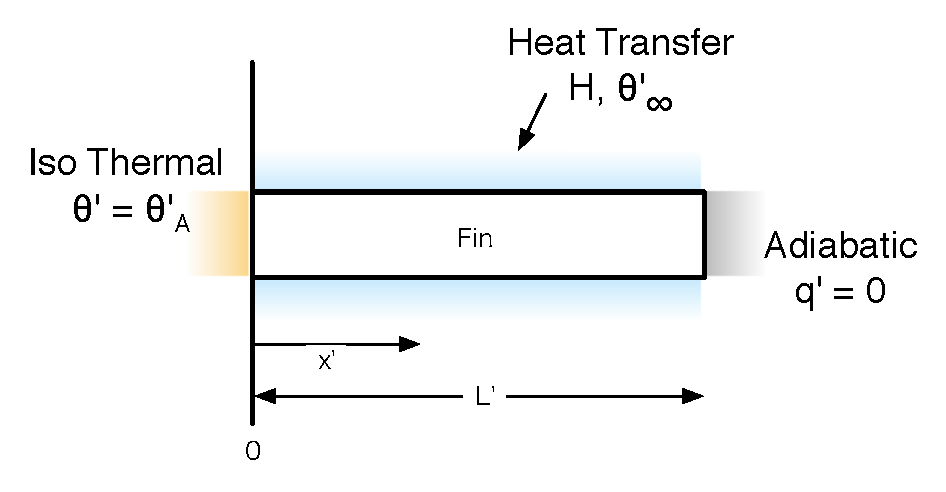
\includegraphics[width=9cm,clip]{1DHC.eps}
\end{center}
\caption{一次元定常熱伝導問題の模式図}
\label{fig:HC1D}
\end{figure}

問題の定式化としては\textbf{式(\ref{eq:shc1d gov eq})}の定常一次元熱伝導の形式となる.
支配方程式は,
\begin{equation}
\frac{d}{d{x}^{\prime}} \left({ \lambda \frac{d \theta^{\prime}}{d{x}^{\prime}} }\right) \,+\,\frac{H P^{\prime}}{A^{\prime}} \left({ {\theta_{\infty}}^{\prime} \,{-}\, \theta^{\prime} }\right)
\,{=}\,{0}
\label{eq:shc1d gov eq}
\end{equation}

\noindent $P',\,A'\,H,\,\lambda$は棒の周囲長さと断面積,熱伝達率,熱伝導率である.
\textbf{式(\ref{eq:shc1d gov eq})}の厳密解は,次式のようになる.
\begin{equation}
\theta
\,=\,
\frac{\theta^{\prime}\,-\,{\theta_{\infty}}^{\prime}} {{\theta_{A}}^{\prime}\,-\,{\theta_{\infty}}^{\prime}}
\,=\,
\frac{\cosh\left[{m\left({{L}{-}{x}}\right)}\right]}{\cosh\left({mL}\right)}{,}
\qquad m\,=\,\sqrt{\frac{H P^{\prime}}{\lambda A^{\prime}}}
\label{eq:1DHE exact solution}
\end{equation}


格子幅が$\Delta x^{\prime}=0.2$の場合には,厳密解のパラメータは,$H=12,\,L^{\prime}=1,\,{\theta_{A}}^{\prime}=200,\,{\theta_{\infty}}^{\prime}=100,\,\lambda=50,\,P^{\prime}=4\Delta x^{\prime},\,A^{\prime}={\Delta x^{\prime}}^2$として計算する.

\paragraph{領域設定}
計算領域は\textbf{図\ref{fig:shc1d dimension}}に示すようにx軸方向に放熱フィンをとり,y,z方向には5つだけセルを設ける.
領域の設定情報として,x方向の分割数をimaxにより与える.
放熱フィンを5分割したい場合には,imax=7を設定する.
$\mathrm{jmax=kmax=5}$で固定である.
このとき,格子幅は$\Delta x = \Delta y = \Delta z = 1\slash \mathrm{(imax-2)}$となる.
計算領域は,$[-\Delta x \sim (\mathrm{imax-1})\Delta x,\, -2.5\Delta y \sim 2.5\Delta y,\,-2.5\Delta z \sim 2.5\Delta z]$となる.

\begin{figure}[htdp]
\begin{center}
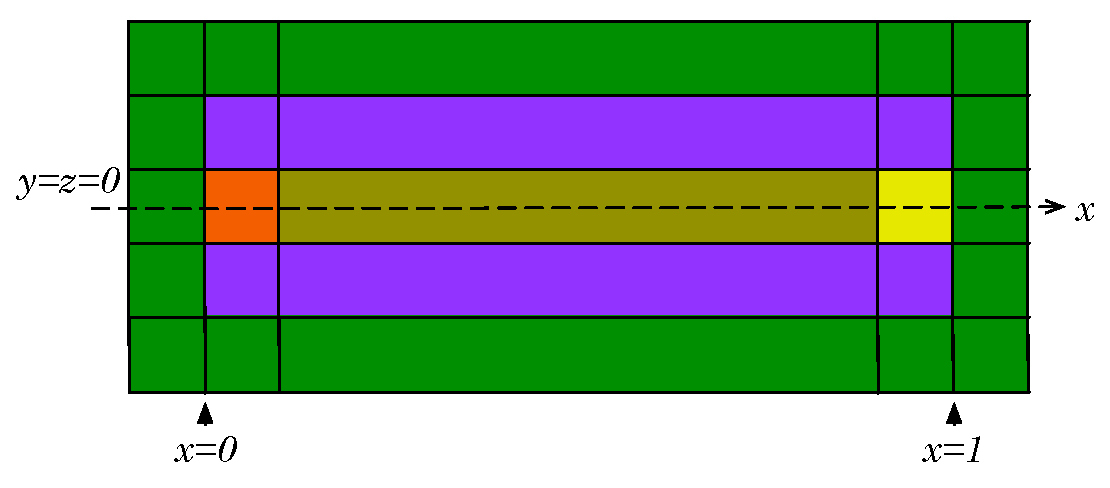
\includegraphics[width=8cm,clip]{dimension.eps}
\end{center}
\caption{計算領域の設定.色は\textbf{表\ref{tbl:set voxel ID}}に対応する.}
\label{fig:shc1d dimension}
\end{figure}

%
\pagebreak
\subsubsection{計算環境}
本計算に利用した計算機環境とソフトウェアを\textbf{表\ref{tbl: shc1d env}}に示す.

\begin{table}[htdp]
\small
\caption{計算機環境および利用ソフトウェア}
\begin{center}
\begin{tabular}{ll}\toprule
Computer & MacBook Pro\\
CPU & Intel Core i7 (2 Cores/CPU)\\
Clock & 2.66 GHz\\
Memory & 8GB\\
Cache(2nd) & 256 KB(each core)\\
Cache(3rd) & 4MB\\ 
OS & Mac OS X 10.6.5\\ \hline
MPI & OpenMPI 1.3.3\\
V-Sphere & ver. 1.8.2\\
CBC & ver. 1.3.0\\
FlowBase & ver. 2.3.0\\ \hline
Compiler & Intel Compiler Composer XE(12.0) C++/Fortran\\
Compile Option & -O3\\
\bottomrule
\end{tabular}
\end{center}
\label{tbl: shc1d env}
\end{table}


%
\subsubsection{解析モデルと計算パラメータ}

本例題は一次元の問題として解けますが,\textbf{図\ref{fig:HC model}}に示すように三次元で計算モデル作成し,三次元非定常熱伝導問題として解く.
この例題は固体熱伝導なので,流体セルは計算しない.

\begin{figure}[htdp]
\begin{minipage}{0.47\hsize}
\begin{center}
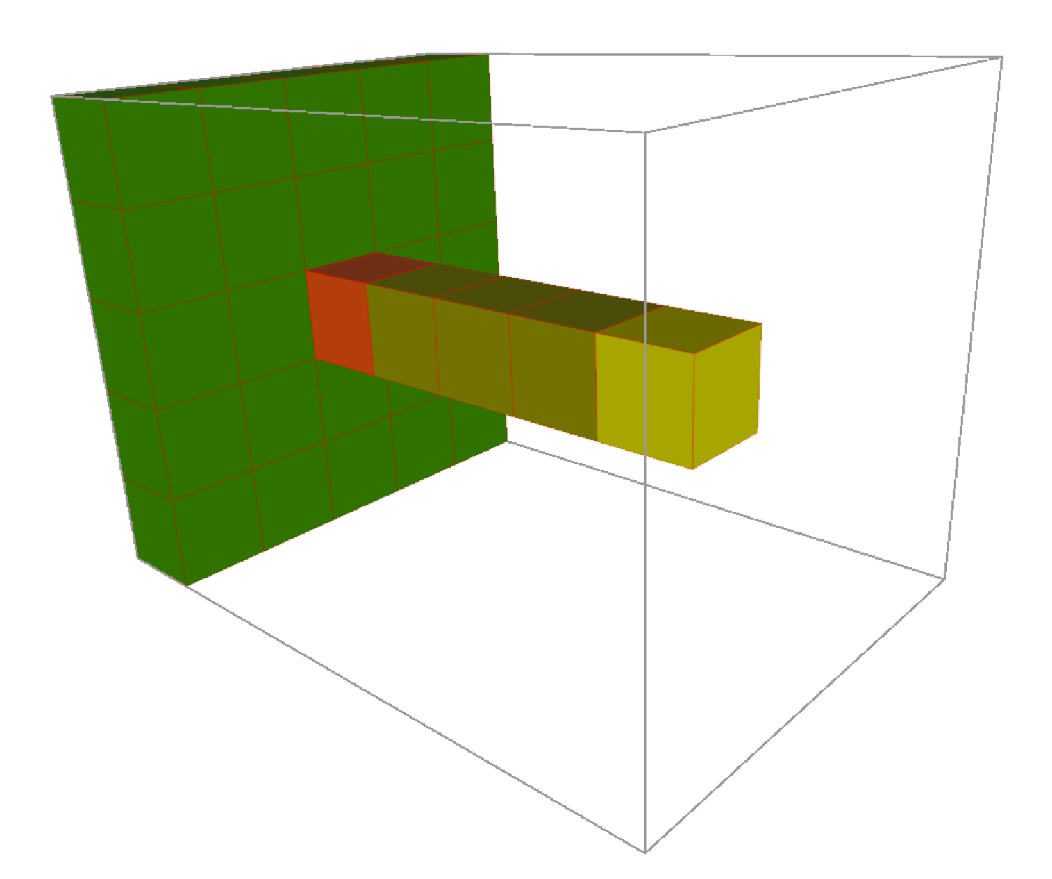
\includegraphics[height=5cm,clip]{model_iso.eps}
\end{center}
\end{minipage}
\begin{minipage}{0.47\hsize}
\begin{center}
\includegraphics[height=5cm,clip]{model_cross.eps}
\end{center}
\end{minipage}
\caption{一次元熱伝導問題を計算するための片持ち梁の三次元モデルとセルID (分割数が$7\times5\times5$の場合)}
\label{fig:HC model}
\end{figure}

計算モデルのセルIDは\textbf{表\ref{tbl:set voxel ID}}のように設定している.

\begin{table}[htdp]
\small
\caption{モデル作成時のID設定}
\begin{center}
\begin{tabular}{llll} \toprule
ID & Color & Medium & Property\\ \midrule
1 & Purple & Fluid & Water\\
500 & Orange & Solid & Iso-thermal wall\\
520 & Yellow & Solid & Adiabatic\\
600 & Green & Solid & Inactive cell\\
610 & Khaki & Solid & Heat conductor\\ \bottomrule
\end{tabular}
\end{center}
\label{tbl:set voxel ID}
\end{table}

計算に用いた物性値を\textbf{表\ref{tbl:shc1d medium_tbl}}に示す.
使用した物性値は物理的なものではなく,無次元のスケールアナリシスから導いた値である.
流体の物性値は実際には使用していない.
XMLパラメータファイルで,問題の指定単位を有次元,温度の単位にCelsiusを指定する.
計算終了時刻は定常状態までの時刻を見て設定している.

{\small
\begin{program}
<Elem name="Unit">
  <Param name="Unit_of_input_parameter" dtype="STRING" value="Dimensional" />
  <Param name="Temperature"             dtype="STRING" value="Celsius" />
</Elem>
\end{program}
}

\begin{table}[htdp]
\small
\caption{計算に用いた物性値}
\begin{center}
\begin{tabular}{llll}\\ \toprule
物性値 & & 流体(ID=1) & 固体(Others)\\ \midrule
密度 & $[kg/m^3]$ & $1.0$ & $1.0$\\
定圧比熱 & $[kJ/(kg K)]$ & $1.0$ & $1.0$\\
熱伝導率 & $[W/(m K)]$ & $1.0$ & $50.0$\\
動粘性係数 & $[m^2/s]$ & $1.0$ &\\
粘性係数 & $[Pa\,s]$ & $1.0$ &\\
音速 & $[m/s]$ & $1.0$ &\\
体膨張率 & $[1/K]$ & $1.0$ &\\ 
\bottomrule
\end{tabular}
\end{center}
\label{tbl:shc1d medium_tbl}
\end{table}


\paragraph{サンプリングの指定}
値のサンプリングは,$y=0,\, z=0$軸上の$x=0.0\sim 1.0$の範囲を分割してサンプリングする.



%
\subsubsection{計算結果と厳密解の比較}

\textbf{図\ref{fig:shc1d compare0}}に$\Delta x=0.2$の場合の無次元化した厳密解と計算結果の比較結果を示す.
5セルの近似であるが,厳密解との誤差は最大2\%であることがわかる.

\begin{figure}[htbp]
\begin{minipage}{.47\textwidth}
\begin{center}
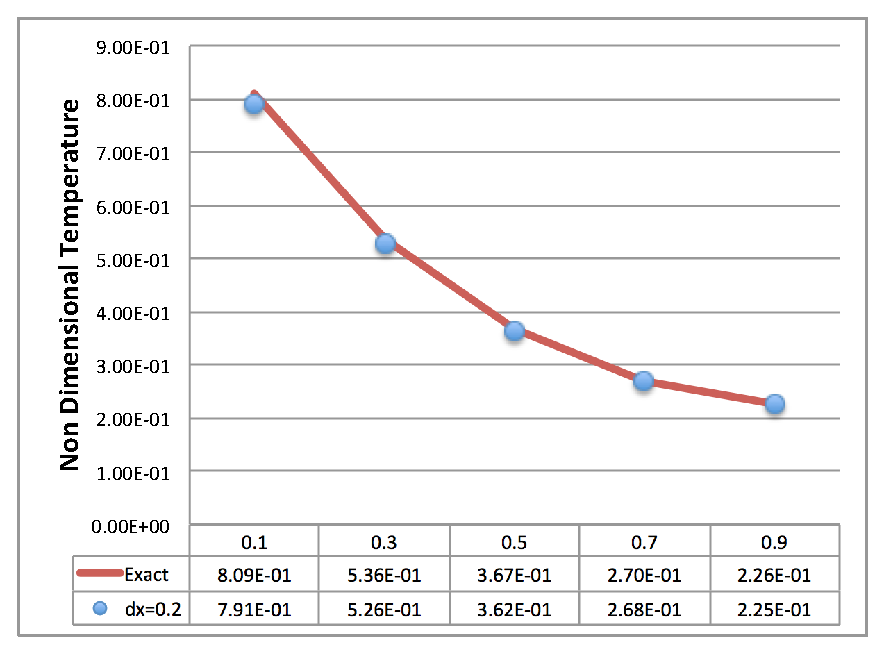
\includegraphics[width=8cm,clip]{cmp_0.eps}
\end{center}
\caption{厳密解と計算結果の比較(Euler陽解法,$\Delta x=0.2 m,\,\Delta t=4.0\times 10^{-4} sec.$, $t=2.48\times 10^{-2} sec.$)}
\label{fig:shc1d compare0}
\end{minipage} \hfill
\begin{minipage}{.47\textwidth}
\begin{center}
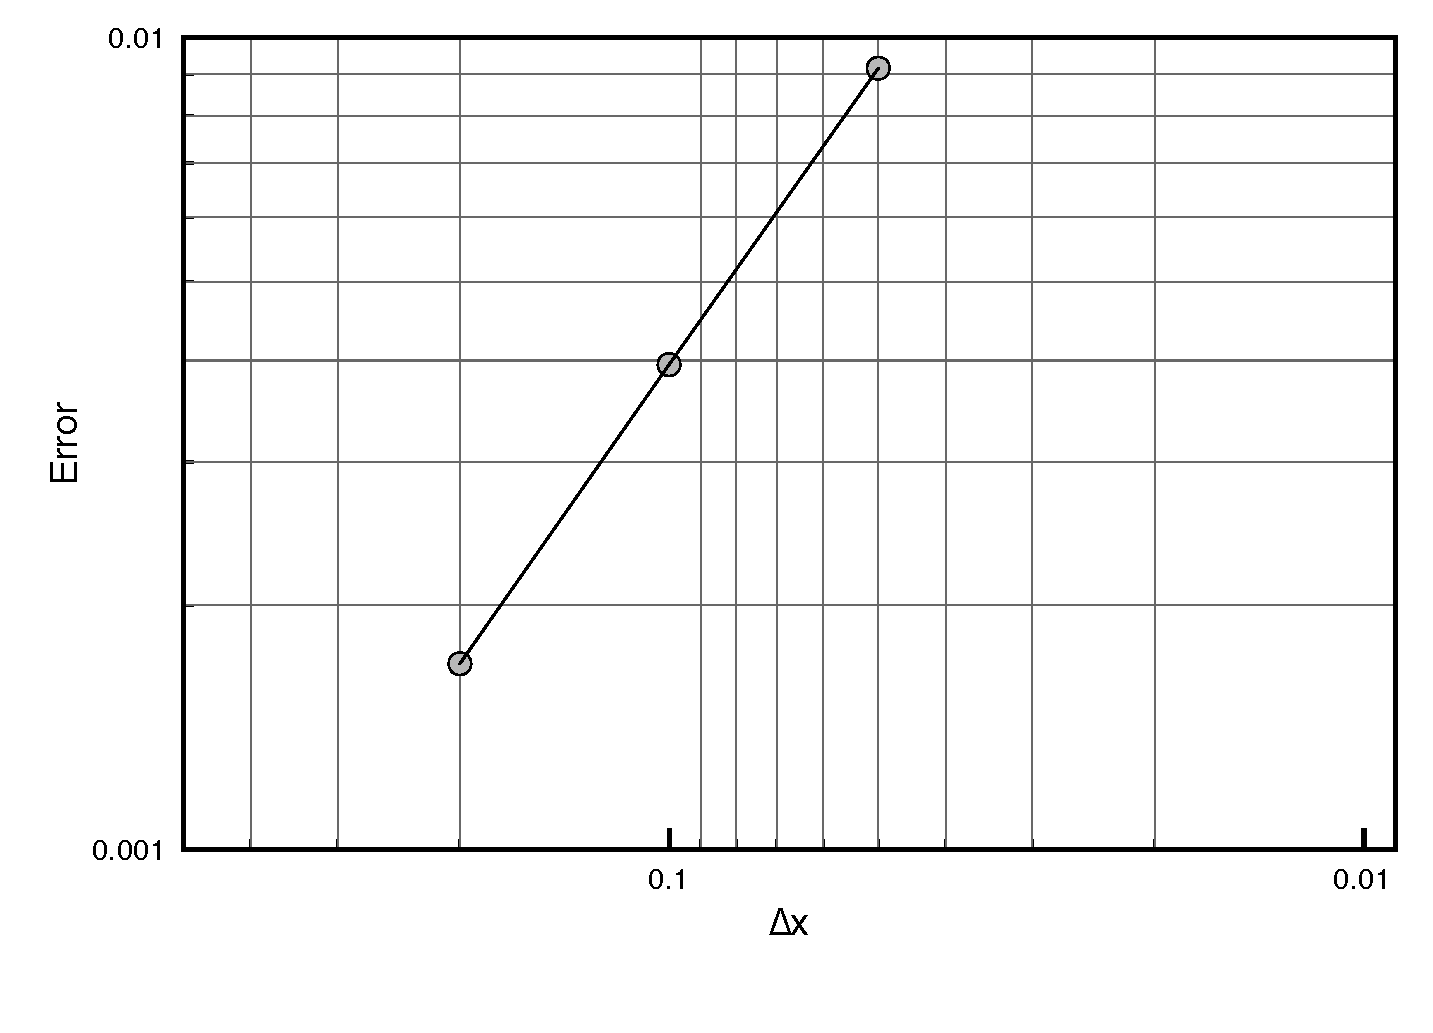
\includegraphics[width=8cm,clip]{error.eps}
\end{center}
\caption{計算結果の格子依存性の比較 ($y=ax^b,\,b=1.21$)}
\label{fig:shc1d compare1}
\end{minipage}
\end{figure}

\textbf{図\ref{fig:shc1d compare1}}には,誤差のメッシュ依存性を示す.グラフの傾きから誤差は格子幅の変化量に対して1.2倍の割合で減少していることがわかる.つまり,この問題の場合には予測精度は1.2次となっている.拡散項のスキームは空間二次精度で離散化されており空間2次精度が期待されるが,境界条件の影響により近似精度が低下している.つまり,等温境界と熱伝達境界の近似精度が一次であるので,この部分の影響を強く受けている.

陽解法では$\Delta t$の値を変化させ,拡散数$D=\lambda \Delta t \slash {\Delta x}^2<1\slash 2$の範囲で安定に計算でき,$D>1\slash 2$では不安定になり発散すること,陰解法では$D\sim 1$程度まで安定に計算できることが確認できる.

%
\pagebreak
\subsubsection{ファイルのメモ}

例題の添付ファイルの説明を以下に示す.ただし,Euler陰解法は$\Delta x=0.2$の場合のみである.

\begin{quote}
\begin{tabbing}
\hspace{18em}\= \hspace{20em}\kill
shc1d\_ee\_\{005, 01, 02\}.xml \> Euler陽解法$\Delta x=0.05,\,0.1,\,0.2$のパラメータ\\
shc1d\_ei\_02.xml \> Euler陰解法$\Delta x=0.2$のパラメータ\\
condition\_*\_\{005, 01, 02\}.txt \> conditionファイル(*=ee:Euler陽解法,ei:Euler陰解法)\\
history\_base\_*\_\{005, 01, 02\}.txt \> history\_baseファイル\\
history\_compo\_*\_\{005, 01, 02\}.txt \> history\_compoファイル\\
sampling\_*\_\{005, 01, 02\}.txt \> samplingファイル\\
comparison.xlsx \> \textbf{図\ref{fig:shc1d compare0}}と\textbf{図\ref{fig:shc1d compare1}}の結果のファイル\\
exact.py \> 厳密解を計算するスクリプトファイル\\
Error.plot \> plotファイル(http://plot.micw.eu/)\\
\end{tabbing}
\end{quote}

\paragraph{厳密解の計算}
exact.pyをエディタで開き,分割数nの値を変更する.実行は以下のようにコマンドラインでタイプすると,対応する結果が表示される.1カラム目がx座標,2カラム目が厳密解である.
{ \small
\begin{program}
$ python exact.py

0.1 0.808704519533
0.3 0.535692813577
0.5 0.367190344487
0.7 0.270323674338
0.9 0.22619491703
\end{program}
}




\graphicspath{{./fig_2Dcouette/}}

\subsection{圧力勾配のある二次元Couette流}
\label{subsection:2Dcouette}

%
\subsubsection{目的}
本例題は,圧力勾配のある二次元のCouette流を,PPLT2D組み込み例題クラスを用いて解析することにより,CBCソルバーの動作検証と予測精度を明らかにする.

%
\subsubsection{問題の定義と厳密解}
いま,二つの平行平板間の定常な流れを考える.平行壁の一方は静止し,他方はUの速度で運動しているとする.圧力勾配のない場合の壁面間のズリ運動による単純せん断流れをCouette(クエット)流れという\cite{imai:73}.ここでは,流れ方向に圧力勾配$dp/dx$が存在する場合のCouette流を計算し,厳密解と比較する\cite{hino:74:fd}.\\

十分に長い平行平板間の流れでは,すべての流体粒子は,一方向に流れ,他の方向の速度成分を持たない.この方向を$x$軸方向,板に垂直な方向を$y$軸とし,これらに垂直に$z$軸をとれば,$v=w=0$であるから,連続の式より明らかに${\partial u}/{\partial x}=0$である.したがって,平行流では,
\begin{equation}
u=u(y, z, t) ; \; v=0; \; w=0
\end{equation}

さらに,Navier-Stokesの方程式の第2,3式より,${\partial p}/{\partial y}=0$,${\partial p}/{\partial z}=0$となるから,圧力$p$は$x$のみの関数である.結局,Navier-Stokesの方程式の第1式より,
\begin{equation}
\rho \frac{\partial u}{\partial t} 
= - \frac{dp}{dx} 
+ \mu \left( \frac{{\partial}^2 u}{\partial y^2}
+ \frac{{\partial}^2 u}{\partial z^2}\right)
\label{eq:NS1}
\end{equation}
が得られる.

いま,二つの平行平板間の定常な流れを考え,平行壁の一方は静止し他方は$U$の速度で運動しているとするとき,
平行壁の間隔を$h$とし,静止壁面上に$x$軸を選べば,運動方程式は,\textbf{式(\ref{eq:NS1})}より,
\begin{equation}
\frac{dp}{dx}=\mu\frac{d^2u}{dy^2}
\label{eq:motion}
\end{equation}
となり,境界条件は,
\begin{equation}
\begin{array}{lll}
y=0 & : & u=0 \\
y=h & : & u=U
\end{array}
\end{equation}
解は次のようになる.
\begin{equation}
u(y)=U\frac{y}{h}-\frac{h^2}{2\mu}\frac{dp}{dx}\frac{y}{h}
\left(1-\frac{y}{h}\right)
\mbox{  }0\leq y\leq h
\end{equation}
無次元圧力勾配を
\begin{equation}
P = \frac{h^2}{2\mu}\frac{1}{U}\left(-\frac{dp}{dx}\right)
\label{eq:P}
\end{equation}
ととると,$P<-1$のとき,$u<0$となる逆流域が生じるようになる(\textbf{図\ref{Fig.couetteG}}).

\begin{figure}[htbp]
\centering
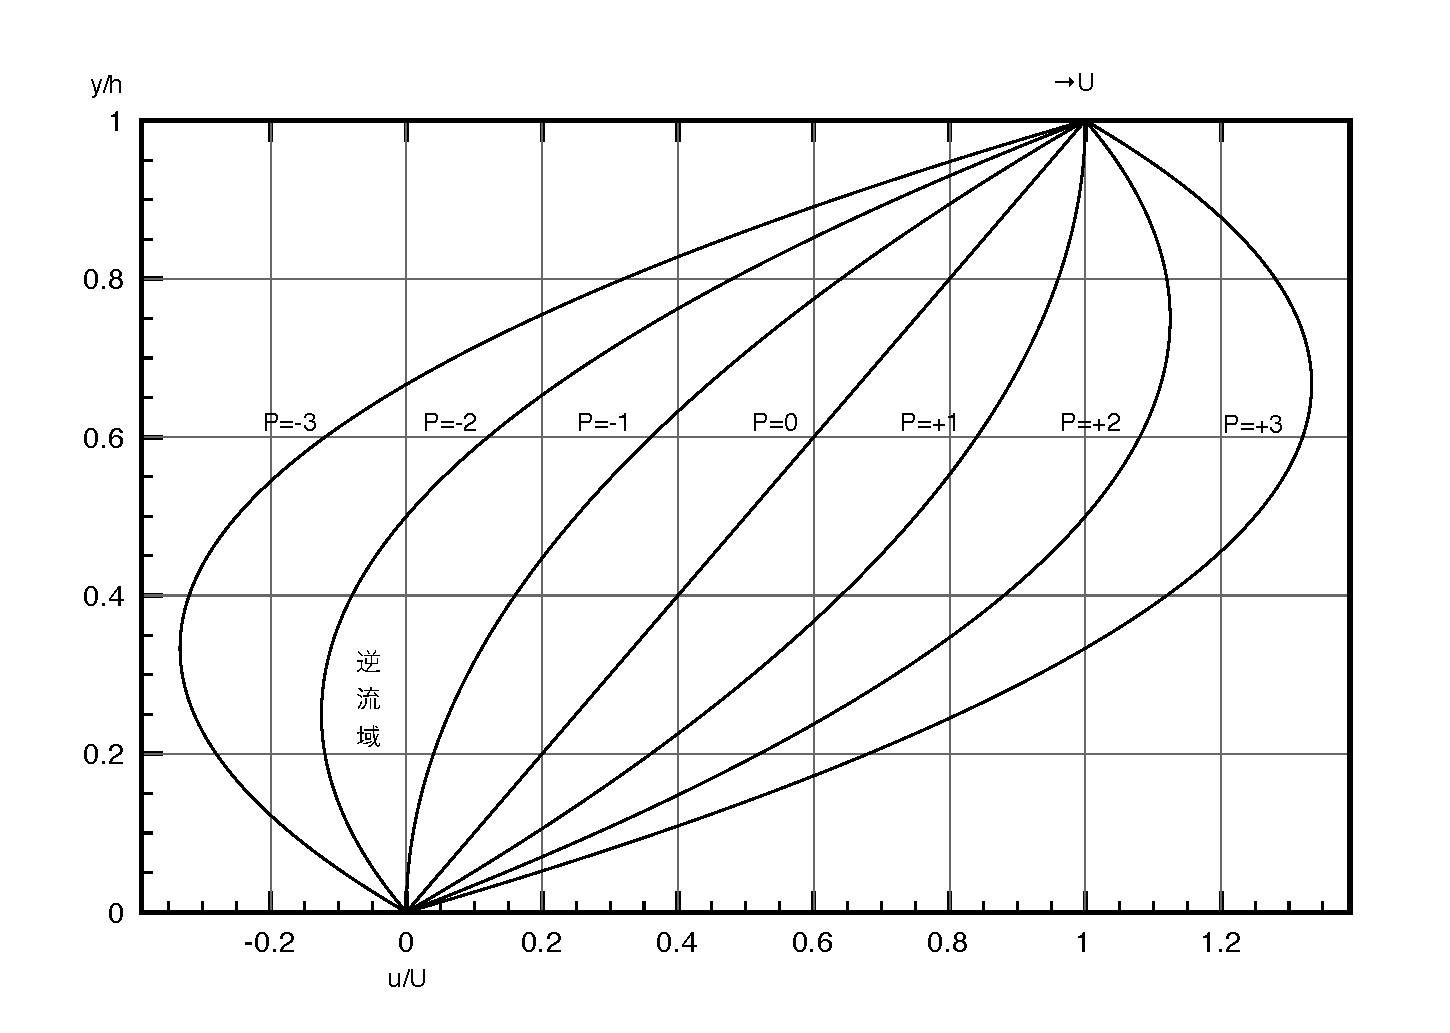
\includegraphics[width=12cm]{exact_solution.eps}
\caption{圧力勾配のある場合のCouette流}
\label{Fig.couetteG}
\end{figure}

\subsubsection{領域設定}
この例題は二次元問題なので,PPLT2D組込例題
クラスを使って計算する.
PPLT2Dクラスは辺長比が2:1の二次元空間を表現する.
$z$方向には3セルを設けており,\textbf{図\ref{Fig.couetteP}}に示すように,単純な周期境界条件を用いて二次元を近似している.
本計算では,$100\times50\times3$のセル分割とした.

コンフィギュレーションファイルの``Example"タグで``Parallel\_Plate\_2D"を指定する.
Couette流を再現するために,$x$軸方向に圧力勾配をかけた周期境界条件を設定し,$y=0$面は固定壁,$y=h$面はスライド($u=U$)壁とみなし,$z\pm$面には単純な周期境界条件を与える.

\begin{figure}[htbp]
\centering
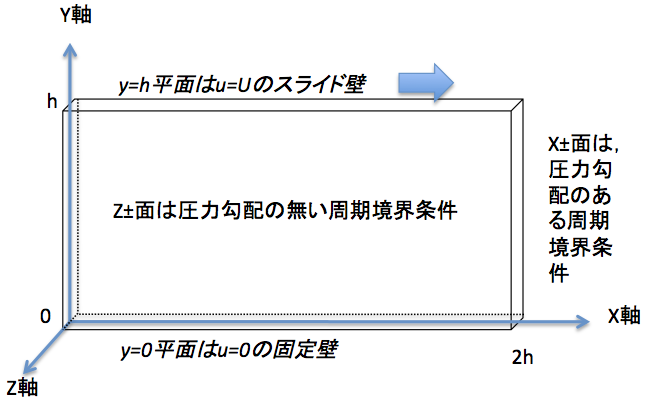
\includegraphics[width=12cm, bb=0 0 646 405]{2Dcouette_model.png}
\caption{計算領域の設定}
\label{Fig.couetteP}
\end{figure}

\pagebreak
\subsubsection{計算環境}
本計算に利用した計算機環境とソフトウェアを\textbf{表\ref{tbl: 2dcouette env}}に示す.

\begin{table}[htdp]
\small
\caption{計算機環境および利用ソフトウェア}
\begin{center}
\begin{tabular}{ll}\toprule
Computer & eX. COMPUTER\\
CPU & Intel Core i7-950 (4 Cores/CPU)$\times$ 2\\
Clock & 3.07 GHz\\
Memory & 12GB \\
Cache & 8 MB(each CPU)\\
%Cache(3rd) & 4MB\\ 
OS & Linux ubuntu 2.6.32-25-generic\\ \hline
MPI & OpenMPI 1.4.3\\
V-Sphere & ver. 1.8.4\\
CBC & ver. 1.3.8\\
FlowBase & ver. 2.3.8\\ \hline
Compiler & Intel Compiler Composer XE(12.0) 2011.3.174 C++/Fortran\\
Compile Option & -O3\\
\bottomrule
\end{tabular}
\end{center}
\label{tbl: 2dcouette env}
\end{table}


%
\subsubsection{計算パラメータ}

計算に用いたパラメータ(\textbf{表\ref{Table.2Dcouette_param}}),流体の物性値(\textbf{表\ref{Table.2Dcouette_bussei}})などを示す.
\begin{table}[htbp]
\centering
\caption{計算に用いたパラメータ}
\label{Table.2Dcouette_param}
\begin{tabular}{llll}\toprule
$h$ &短辺の長さ &$1.0$ &[m]\\
$U$ &$y=h$の壁面の移動速度 & $1.0$ &[m/s]\\
$\Delta p$ &$x\pm$面間の圧力差($P=1$に相当) &$4.7052\times10^{-2}$ &[Pa]\\
$\nu $ & クーラン数 & 0.2& \\
\bottomrule
\end{tabular}
\end{table}

\begin{table}[htbp]
\centering
\caption{計算に用いた物性値}
\label{Table.2Dcouette_bussei}
\begin{tabular}{llll}\toprule
物性 &&物性値  & [単位]\\
\midrule
$\rho$ & 密度 & 1.1763 & [kg/m$^3$]\\
$\mu$  & 粘性係数 & 1.1763 $\times 10^{-2}$ &[Pa $\cdot$ s]\\
\bottomrule
\end{tabular}
\end{table}

\textbf{表\ref{Table.2Dcouette_param}},\textbf{表\ref{Table.2Dcouette_bussei}}から,レイノルズ数は,Re=$\rho U h/\mu=100$となる.
レイリーの問題から,時間$t$[s]の間に壁の影響が粘性を通じて及ぶ距離$\delta$[m]は,$\delta=\sqrt{t\nu}$.$\nu$は動粘性係数[m$^2$/s].無次元にすると$t^*=\delta^{*2}\cdot Re$となり,$\delta^*=1$,Re=100より,計算時間をt=100[-]と見積もった.

\paragraph{サンプリングの指定}
値のサンプリングは,$z=0, x=h$上の$y=0 \sim h$の範囲を分割してサンプリングする.今回の計算では,分割数を25とした.

\paragraph{外部境界条件}コンフィギュレーションファイルの中で,外部境界条件において,圧力勾配($P=+1$)をかける周期境界条件と,圧力勾配をかけない周期境界条件($z\pm$面)を設定する様子を示す.
{\small
\begin{program}
    <OuterBoundary>
      <Elem name="Basic_BCs">
        <Elem name="Wall" id="1">
            <Param dtype="REAL" name="Normal_X" value="0.0"/>
            <Param dtype="REAL" name="Normal_Y" value="0.0"/>
            <Param dtype="REAL" name="Normal_Z" value="0.0"/>
            <Param dtype="STRING" name="Specified_Type" value="Velocity"/>
            <Param dtype="STRING" name="Profile" value="Constant"/>
            <Param dtype="REAL" name="Specified_Value" value="0.0"/>
        </Elem>
        <Elem name="Wall" id="2">
            <Param dtype="REAL" name="Normal_X" value="1.0"/>
            <Param dtype="REAL" name="Normal_Y" value="0.0"/>
            <Param dtype="REAL" name="Normal_Z" value="0.0"/>
            <Param dtype="STRING" name="Specified_Type" value="Velocity"/>
            <Param dtype="STRING" name="Profile" value="Constant"/>
            <Param dtype="REAL" name="Specified_Value" value="1.0"/>
        </Elem>
        <Elem name="periodic" id="7" >
          <Param name="mode" dtype="string" value="simple_copy" />
        </Elem>
        <Elem name="periodic" id="8" >
          <Param name="mode" dtype="string" value="Directional" />
          <Param name="pressure_difference" dtype="REAL" value="0.047052" />
          <Param name="flow_direction" dtype="string" value="upstream" />
        </Elem>
        <Elem name="periodic" id="9" >
          <Param name="mode" dtype="string" value="Directional" />
          <Param name="pressure_difference" dtype="REAL" value="0.047052" />
          <Param name="flow_direction" dtype="string" value="downstream" />
        </Elem>
      </Elem>
	
      <Elem name="Face_BC">
        <Elem name="X_MINUS" id="8" comment="periodic_upstream">
          <Param name="Guide_Cell_ID" id="1" />
        </Elem>
        <Elem name="X_PLUS"  id="9" comment="periodic_downstream">
          <Param name="Guide_Cell_ID" id="1" />
        </Elem>
        <Elem name="Y_MINUS" id="1" comment="wall">
          <Param name="Guide_Cell_ID" id="600" />
        </Elem>
        <Elem name="Y_PLUS"  id="2" comment="slidewall">
          <Param name="Guide_Cell_ID" id="600" />
        </Elem>
        <Elem name="Z_MINUS" id="7" comment="periodic">
          <Param name="Guide_Cell_ID" id="1" />
        </Elem>
        <Elem name="Z_PLUS"  id="7" comment="periodic">
          <Param name="Guide_Cell_ID" id="1" />
        </Elem>
      </Elem>
    </OuterBoundary>
\end{program}
}

%
\subsubsection{計算結果と厳密解の比較}
\textbf{図\ref{Fig.couette_exact_100}}に,無次元圧力勾配$P=-3, -2, -1, 0, +1, +2, +3$の場合の,厳密解(実線)およびCBCの計算結果$u/U$(マーク)の値を比較した.CBCと厳密解の誤差は,厳密解の0.01\%以内に収まっており,よく一致しているといえる.


\begin{figure}[htbp]
\begin{center}
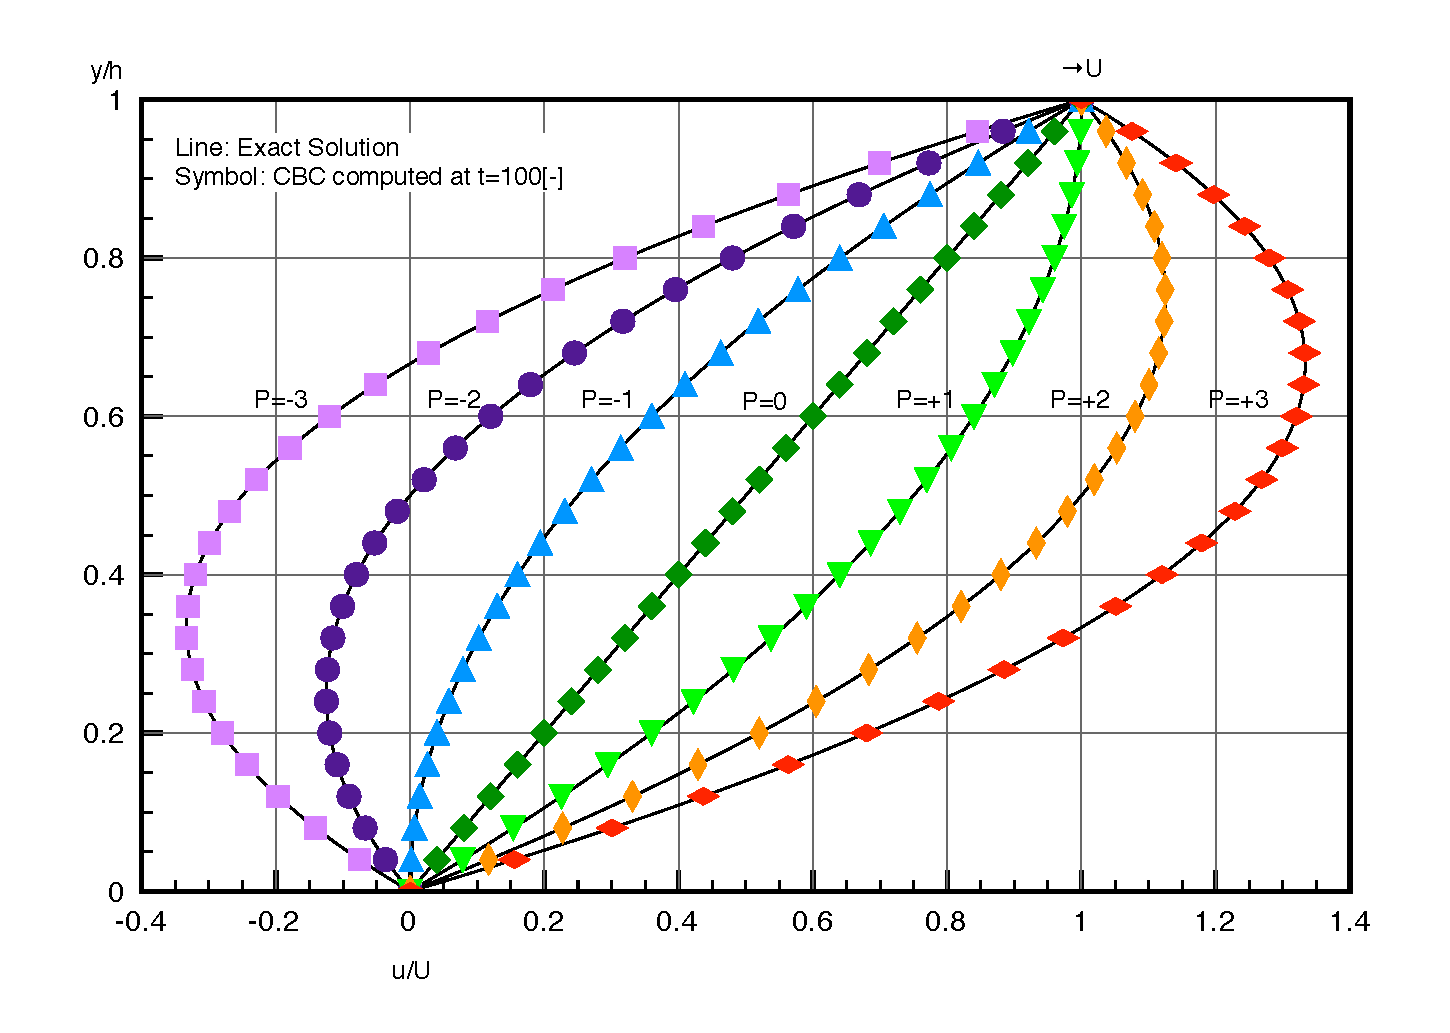
\includegraphics[width=14cm]{exact_100.eps}
\end{center}
\caption{圧力勾配のあるCouette流の速度分布(厳密解とCBCシミュレーションの比較)}
\label{Fig.couette_exact_100}
\end{figure}

%
\subsubsection{ファイルのメモ}
例題の提供ファイルの説明を以下に示す.\\
%\begin{quote}
\begin{tabularx}{180mm}{lclclX}
%\hspace{12em}\= \hspace{30em}\kill
example\CID{07480}2Dcouette & \CID{07530}&\CID{00718}&\CID{07530}&couette.xml & 圧力勾配$*:P=-3,\,-2,\,-1,\,0,\,1,\,2,\,3$の場合のコンフィギュレーションファイル\\
&\CID{07482}&&\CID{07514}&condition.txt & conditionファイル
\\
&\CID{07482}&&\CID{07514}&profiling.txt & 実行時性能測定結果ファイル\\
&\CID{07482}&&\CID{07514}&sample\_x=0.log& samplingファイル\\
&\CID{07482}&&\CID{07502}&history\_base.log&履歴ファイル\\
%&\CID{07482}&&\CID{07502}&(error\_P=+3.plot) & $P=+3$における解析解と厳密解との誤差.図\ref{Fig.couette.error} (\url{http://plot.micw.eu/})
%\\
%&\CID{07514}&\multicolumn{3}{l}{exact.f90} & 厳密解を計算するFortranコード\\
&\CID{07502}&\multicolumn{3}{l}{exact\_100.plot} &  厳密解と,$t=100[-]$における解析解の比較.\textbf{図\ref{Fig.couette_exact_100}}\\
& & &&&(\url{http://plot.micw.eu/})
\end{tabularx}
\\
\paragraph{conditionファイル内の無次元圧力勾配について}
condition.txtファイルの\lq\lq Outer Boundary Conditions\rq\rq セクションに,
周期境界条件に関連して,圧力差と圧力勾配の有次元値と無次元値が記載されている.
CBCではこの無次元化について,「圧力勾配のあるCouette流」に特有の\textbf{式(\ref{eq:P})}を使わず,通常Navier-Stokes方程式で使われる無次元化$p^*=p/(\rho U^2)$,$x^*=x/L$,$(dp/dx)^*=(dp/dx)\,L/(\rho U^2)$を用いている.そのため,圧力勾配$P=a$のcondition.txtファイルのPressure Gradientの無次元値が$a$と異なる値になっている.

具体的に,無次元圧力勾配$P=1$の場合を示すと,
{\small
\begin{verbatim}
	>> Outer Boundary Conditions

	      Set X- up as Periodic : (periodic_upstream)
       Guide Cell ID = 1 / Medium = 800
       Pressure Difference = 4.705200e-02 [Pa]    /  4.000000e-02 [-]
       Pressure Gradient   = 2.352600e-02 [Pa/m]  /  2.000000e-02 [-]

	      Set X+ up as Periodic : (periodic_downstream)
       Guide Cell ID = 1 / Medium = 800
       Pressure Difference = 4.705200e-02 [Pa]    /  4.000000e-02 [-]
       Pressure Gradient   = 2.352600e-02 [Pa/m]  /  2.000000e-02 [-]
\end{verbatim}
}

圧力勾配の無次元化は,\textbf{式(\ref{eq:P})}に従うと,
\[
P=\frac{h^2}{2\mu}\frac{1}{U}\left(-\frac{dp}{dx}\right)
  =\frac{1.0[m^2]}{2\times 1.1763\times10^{-2}[Pa\cdot s]\times 1.0[m \cdot s^{-1}]}\times 2.3526 \times 10^{-2}[Pa\cdot m^{-1}]
=1.0000[-]
\]
通常の無次元化を用いると,
\[
\left(\frac{dp}{dx}\right)^*=\frac{dp}{dx}\frac{L}{\rho U^2}
=2.3526 \times 10^{-2}[Pa\cdot m^{-1}]\times 
\frac{1.0[m]}{1.1763 \times 10^{-2}[Pa\cdot s] \times 1.0[m^2]}
=2.0000\times 10^{-2}[-]
\]
のようになる.

%\end{quote}




\graphicspath{{./fig_2Dpoiseuille/}}

\subsection{二次元Poiseuille流}

%
\subsubsection{目的}
本例題は,二次元のPoiseuille流をPPLT2D組み込み例題クラスを用いて解析することにより,CBCソルバーの動作検証と予測精度を明らかにする.

%
\subsubsection{問題の定義と厳密解}
いま,2枚の平行平板間の定常な流れを考える.2枚の板を固定して,圧力勾配によって流体を押し流すときの流れを二次元のPoiseuilleの流れ(two-dimensional Poiseuille flow)という\cite{imai:73}.\\

平行平板の間隔を$h$とし,静止壁面上に$x$軸を選べば,運動方程式は,\ref{subsection:2Dcouette}圧力勾配のある二次元Couette流の場合と同じく,
\begin{equation}
\frac{dp}{dx}=\mu\frac{d^2u}{dy^2}
\end{equation}
となり,境界条件は,
\begin{equation}
\begin{array}{lll}
y=0 & : & u=0 \\
y=h & : & u=0
\end{array}
\end{equation}
解は次のようになる.
\begin{equation}
u(y)=-\frac{h^2}{2\mu}\frac{dp}{dx}\frac{y}{h}
\left(1-\frac{y}{h}\right)
\mbox{  }0\leq y\leq h
\end{equation}

平板間の中心線$y=h/2$に関して対称な放物線形の速度分布を持つ(\textbf{図\ref{Fig.poiseuilleG}}).
図中の$P$は無次元圧力勾配

\begin{equation}
P = \frac{h^2}{2\mu}\frac{1}{U}\left(-\frac{dp}{dx}\right)
\end{equation}
である.

\begin{figure}[htbp]
\centering
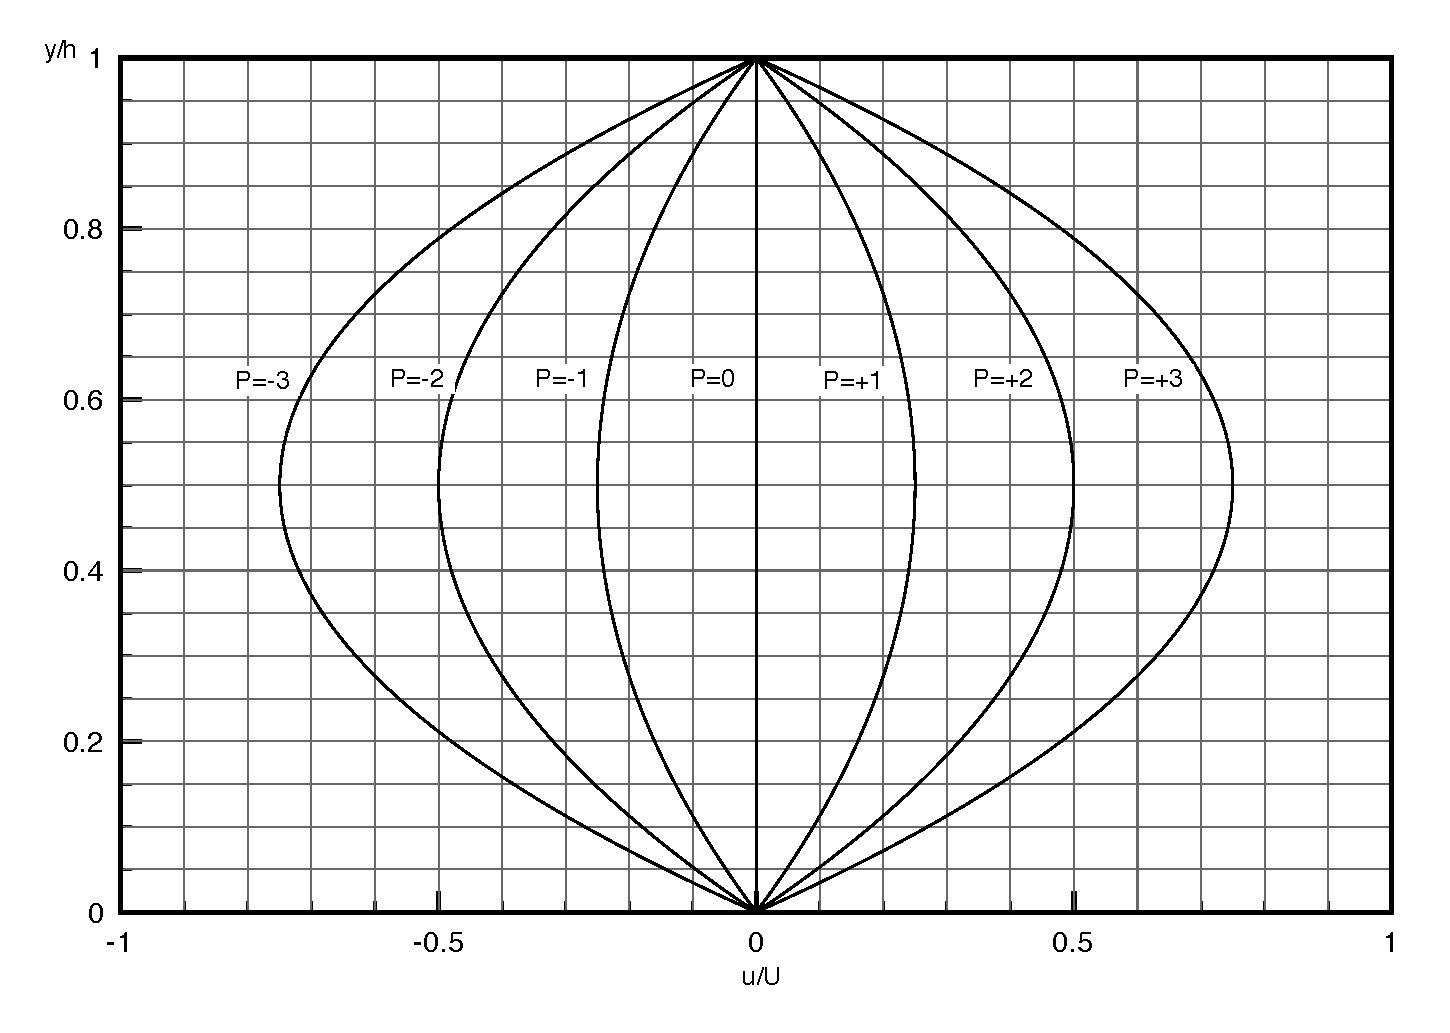
\includegraphics[width=12cm]{2DpoiseuilleG.eps}
\caption{二次元のPoiseuille流の圧力勾配に対する流速分布}
\label{Fig.poiseuilleG}
\end{figure}

\subsubsection{領域設定}
PPLT2Dクラスは辺長比が2:1の二次元空間を表現する.
$z$方向には3セルを設けており,\textbf{図\ref{Fig.poiseuilleP}}に示すように,単純な周期境界条件を用いて二次元を近似している.
本計算では,$100\times50\times3$のセル分割とした.

コンフィギュレーションファイルの\lq\lq Example\rq\rq タグで\lq\lq Parallel\_Plate\_2D\rq\rq を指定する.
Poiseuille流を再現するために,$x$軸方向に圧力勾配をかけた周期境界条件を設定し,$y=0$面,$y=h$面はは固定壁とみなし,$z\pm$面には単純な周期境界条件を与える.

\begin{figure}[htbp]
\centering
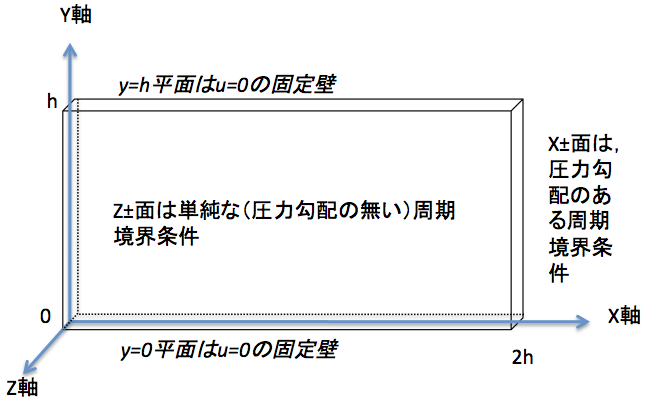
\includegraphics[width=12cm, bb=0 0 647 404]{model.png}
\caption{計算領域の設定}
\label{Fig.poiseuilleP}
\end{figure}

%\pagebreak
\subsubsection{計算環境}
本計算に利用した計算機環境とソフトウェアを\textbf{表\ref{tbl: 2dpoiseuille env}}に示す.

\begin{table}[htdp]
\small
\caption{計算機環境および利用ソフトウェア}
\begin{center}
\begin{tabular}{ll}\toprule
Computer & eX. COMPUTER\\
CPU & Intel Core i7-950 (4 Cores/CPU)$\times$ 2\\
Clock & 3.07 GHz\\
Memory & 12GB \\
Cache & 8 MB(each CPU)\\
%Cache(3rd) & 4MB\\ 
OS & Linux ubuntu 2.6.32-25-generic\\ \hline
MPI & OpenMPI 1.4.3\\
V-Sphere & ver. 1.8.4\\
CBC & ver. 1.3.8\\
FlowBase & ver. 2.3.8\\ \hline
Compiler & Intel Compiler Composer XE(12.0) 2011.3.174 C++/Fortran\\
Compile Option & -O3\\
\bottomrule
\end{tabular}
\end{center}
\label{tbl: 2dpoiseuille env}
\end{table}


%
\subsubsection{計算パラメータ}
計算に用いたパラメータ(\textbf{表\ref{Table.poi_param}}),流体の物性値(\textbf{表\ref{Table.poi_bussei}})などを示す.
\begin{table}[htbp]
\centering
\caption{計算に用いたパラメータ}
\label{Table.poi_param}
\begin{tabular}{llll}\toprule
$h$ &短辺の長さ &$1.0$ &[m]\\
$U$ &代表速度 & $1.0$ &[m/s]\\
$\Delta p$ &$x\pm$面間の圧力差($P=1$に相当) &$4.7052\times10^{-2}$ &[Pa]\\
$\nu $ & クーラン数 & 0.2 & \\
\bottomrule
\end{tabular}
\end{table}

\begin{table}[htbp]
\centering
\caption{計算に用いた物性値}
\label{Table.poi_bussei}
\begin{tabular}{llll}\toprule
物性 &&物性値  & [単位]\\
\midrule
$\rho$ & 密度 & 1.1763 & kg/m$^3$\\
$\mu$  & 粘性係数 & 1.1763 $\times 10^{-2}$ &[Pa $\cdot$ s]\\
\bottomrule
\end{tabular}
\end{table}

\textbf{表\ref{Table.poi_param}},\textbf{表\ref{Table.poi_bussei}}から,レイノルズ数は,Re=$\rho U h/\mu=100$となる.
レイリーの問題から,時間$t$[s]の間に壁の影響が粘性を通じて及ぶ距離$\delta$[m]は,$\delta=\sqrt{t\nu}$.$\nu$は動粘性係数[m$^2$/s].無次元にすると$t^*=\delta^{*2}\cdot Re$となり,$\delta^*=1$,Re=100より,計算時間をt=100[-]と見積もった.

\paragraph{サンプリングの指定}
値のサンプリングは,$z=h/2, x=h$上の$y=0 \sim h$の範囲を分割してサンプリングする.今回の計算では,分割数を25とした.

\paragraph{外部境界条件}コンフィギュレーションファイルの中で,外部境界条件において,圧力勾配($P=+1$)をかける周期境界条件と,単純な周期境界条件($z\pm$面)を設定する指定内容を示す.
{\small
\begin{program}
         <OuterBoundary>
            <Elem name="Basic_BCs">
                <Elem id="1" name="Wall">
                    <Param dtype="REAL" name="Normal_X" value="0.0"/>
                    <Param dtype="REAL" name="Normal_Y" value="0.0"/>
                    <Param dtype="REAL" name="Normal_Z" value="0.0"/>
                    <Param dtype="STRING" name="Specified_Type" value="Velocity"/>
                    <Param dtype="STRING" name="Profile" value="Constant"/>
                    <Param dtype="REAL" name="Specified_Value" value="0.0"/>
                </Elem>
                <Elem id="7" name="periodic">
                    <Param dtype="STRING" name="mode" value="Simple_Copy"/>
                </Elem>
                <Elem id="8" name="periodic">
                    <Param dtype="STRING" name="mode" value="Directional"/>
                    <Param dtype="STRING" name="flow_direction" value="upstream"/>
                    <Param dtype="REAL" name="pressure_difference" value="0.047052"/>
                </Elem>
                <Elem id="9" name="periodic">
                    <Param dtype="STRING" name="mode" value="Directional"/>
                    <Param dtype="STRING" name="flow_direction" value="downstream"/>
                    <Param dtype="REAL" name="pressure_difference" value="0.047052"/>
                </Elem>
            </Elem>
            <Elem name="Face_BC">
                <Elem comment="periodic_u" id="8" name="X_minus">
                    <Param id="600" name="Cell_ID"/>
                </Elem>
                <Elem comment="periodic_d" id="9" name="X_plus">
                    <Param id="600" name="Cell_ID"/>
                </Elem>
                <Elem comment="wall" id="1" name="Y_minus">
                    <Param id="600" name="Cell_ID"/>
                </Elem>
                <Elem comment="slide_wall" id="1" name="Y_plus">
                    <Param id="600" name="Cell_ID"/>
                </Elem>
                <Elem comment="periodic" id="7" name="Z_minus">
                    <Param id="600" name="Cell_ID"/>
                </Elem>
                <Elem comment="periodic" id="7" name="Z_plus">
                    <Param id="600" name="Cell_ID"/>
                </Elem>
            </Elem>
       </OuterBoundary>
\end{program}
}


%
\subsubsection{計算結果と厳密解の比較}

図\ref{Fig.poi_exact_100}に,無次元圧力勾配$P=-3, -2, -1, 0, +1, +2, +3$の場合の,厳密解(実線)およびCBCの計算結果$u/U$(マーク)の値を比較した.
CBCと厳密解の誤差は,厳密解の$10^{-4}$のオーダーに収まっており,よく一致しているといえる.


\begin{figure}[htbp]
\begin{center}
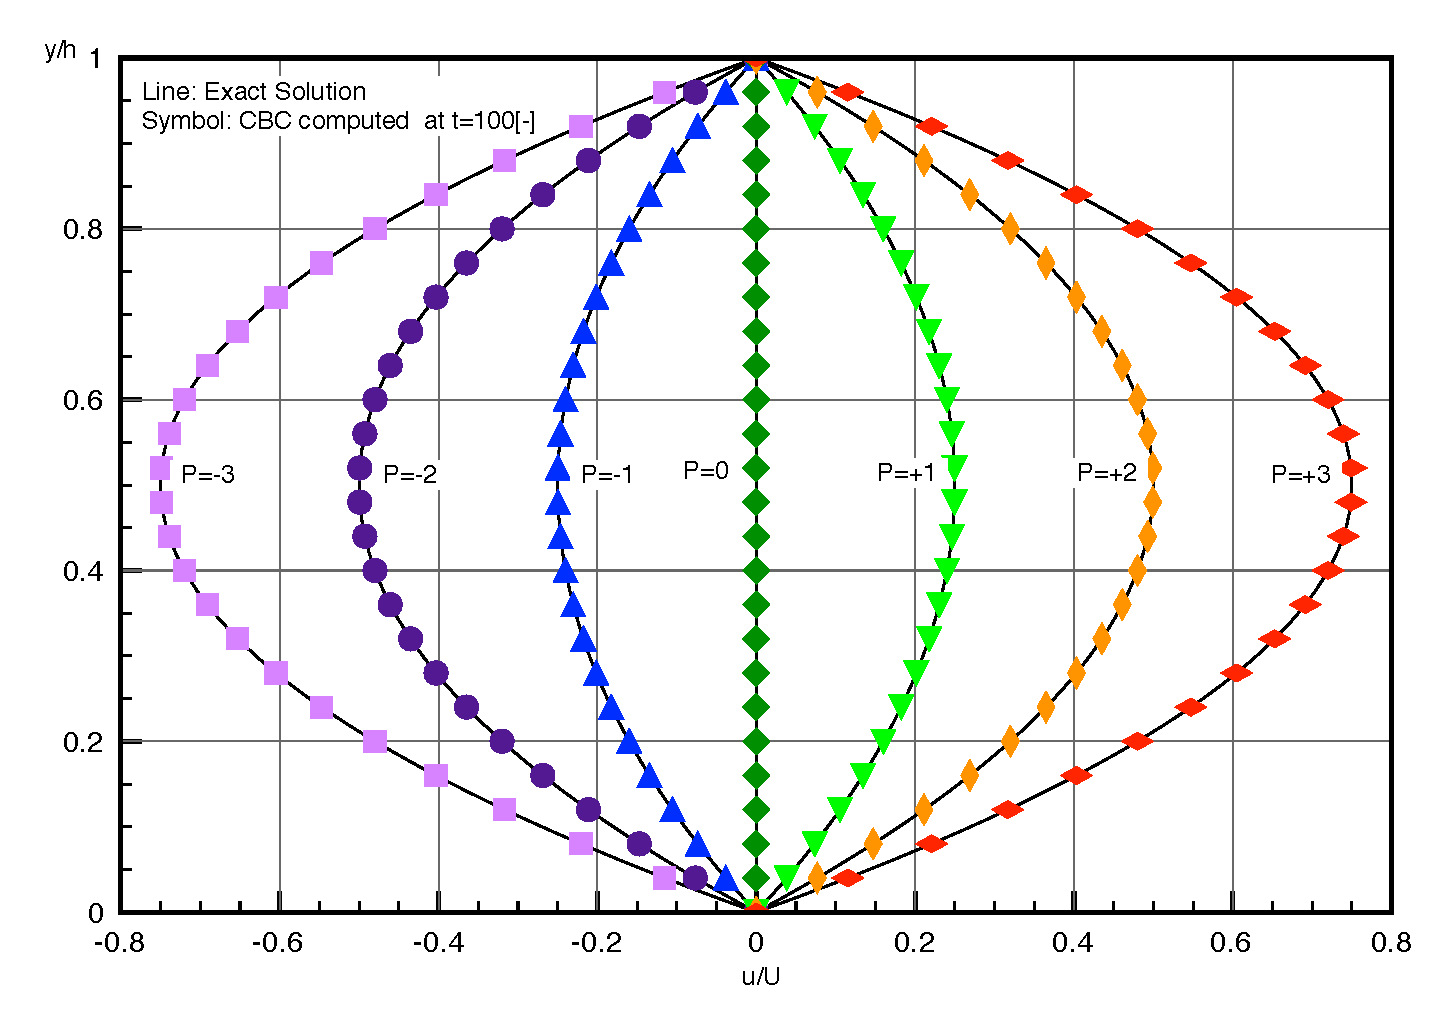
\includegraphics[width=14cm]{2Dpoiseuille_100.eps}
\end{center}
\caption{Poiseuille流の速度分布(厳密解とシミュレーションの比較)}
\label{Fig.poi_exact_100}
\end{figure}

%
\subsubsection{ファイルのメモ}
例題の提供ファイルの説明を以下に示す.\\
%\begin{quote}
%\centering
\begin{tabularx}{180mm}{lclclX}
%\hspace{12em}\= \hspace{30em}\kill
example\CID{07480}2Dpoiseuille & \CID{07530}&\CID{00718}&\CID{07530}&poiseuille.xml & 圧力勾配$*:P=-3,\,-2,\,-1,\,0,\,1,\,2,\,3$の場合のコンフィギュレーションファイル\\
&\CID{07482}&&\CID{07514}&condition.txt & conditionファイル\\
&\CID{07482}&&\CID{07514}&profiling.txt & 実行時性能測定結果ファイル\\
&\CID{07482}&&\CID{07514}&sample\_x=0.log & samplingファイル\\
&\CID{07482}&&\CID{07502}&history\_base.log& 履歴ファイル\\
%&\CID{07482}&&\CID{07502}&(error\_P=+3.plot) & $P=+3$における解析解と厳密解との誤差.図\ref{Fig.couette.error} (\url{http://plot.micw.eu/})
%\\
%&\CID{07514}&\multicolumn{3}{l}{exact.f90} & 厳密解を計算するFortranコード\\
&\CID{07502}&\multicolumn{3}{l}{2Dpoiseuille\_100.plot} &  厳密解と,$t=100[-]$における解析解の比較.\textbf{図\ref{Fig.poi_exact_100}}\\
& & &&&(\url{http://plot.micw.eu/})
\end{tabularx}
%\end{quote}
\\
\paragraph{conditionファイル内の無次元圧力勾配について}
{}~\ref{subsection:2Dcouette}圧力勾配のある二次元Couette流の同項目を参照.

%%
\section{非定常問題}
非定常の厳密解をもつ問題として,以下の例題を示します.
\begin{enumerate}
\item Rayleigh流れ
\item Stokesの第二問題
\end{enumerate}

%
%\include{RayleighFlow}

\graphicspath{{./fig_stokes2nd/}}

\subsection{振動平板による流れ: Stokesの第二問題}

\subsubsection{目的}
本例題は,無限に広い平板が粘性流体の中で振動するときに,引き起こされる流体の運動\cite{hino:74:fd, imai:73}(Stokesの第二問題)について,CBCソルバーの動作検証と予測精度を明らかにする.なお,本例題は,組込例題「Rect」クラスの2次元を用いる.

\subsubsection{問題の定義と厳密解}
いま,無限に広い平板が無限に広がっている粘性流体の中で自分自身に平行に単振動をしている場合を考える.
平板の振動方向に$x$軸をとり,平板自身は$xz$平面内で運動するものとすれば,それによって引き起こされる流体の運動は$x$軸に平行である.

Navier-Stokesの方程式から導かれる,この場合の基礎方程式は,
\begin{equation}
\frac{\partial u}{\partial t} = \nu \frac{\partial^2 u}{\partial y^2},\mbox{  } y>0
\label{eq:kiso}
\end{equation}
となる(平板の片側の半無限の領域$y>0$を考える).

境界条件は,

\begin{equation}
\begin{array}{lcl}
y \rightarrow \infty & : & u \rightarrow 0 \\
y = 0 & : & u = U cos (\omega t)
\end{array}
\label{eq:kyokai}
\end{equation}

具体的には
境界条件$y=0$の速度を

\begin{equation}
y=0\mbox{ }:\mbox{ }u=U e^{i \omega t}
\label{eq:kyokai_e}
\end{equation}

と置き換え,得られた結果の実数部
$Re(u)$をとればよい.

$u$は,$y$の関数と考えられるので,$u$の解の形として,

\begin{equation*}
u=f(y)e^{i \omega t}
\end{equation*}

を求めることにする.これを\textbf{式(\ref{eq:kiso})}に代入すると,

\begin{equation*}
\frac{d^2 f}{dy^2}=\frac{i \omega}{\nu}f
\end{equation*}

の二階常微分方程式が求まり,その一般解は,

\begin{equation*}
f=Ae^{\lambda y} + B e^{-\lambda y}, \mbox{  }A, \, B\mbox{は任意定数}
\end{equation*}

の形に与えられる.ただし,

\begin{equation*}
\lambda=\sqrt{\frac{i \omega}{\nu}}
=\sqrt{i}\sqrt{\frac{\omega}{\nu}}
=\frac{1+i}{\sqrt{2}}\sqrt{\frac{\omega}{\nu}}
=(1+i)\,k, \mbox{ ここで}
k=\sqrt{\frac{\omega}{2\nu}}
\end{equation*}

である.$y \rightarrow \infty$に対して,$e^{\lambda y} \rightarrow \infty$であるから,境界条件(\ref{eq:kyokai})から$A=0$.また境界条件(\ref{eq:kyokai_e})から,$B=U$が得られる.したがって,

\begin{eqnarray*}
u & = & Re \left(f(y)e^{i \omega t}\right) 
=Re\left(U e^{-\lambda y} e^{i\omega t }\right)
= Re \left(U e^{-ky}e^{i(\omega t - ky)}\right) \nonumber\\
 & = & U e^{-ky}cos (\omega t - ky)
\end{eqnarray*}

が求める解である.これは$y$方向に伝わる減衰性の正弦波で,その位相速度は,

\begin{equation*}
c=\frac{\omega}{k}=\sqrt{2 \omega \nu}
\end{equation*}

で与えられる.波数および減衰定数はともに$k=\sqrt{\omega/2\nu}$である.したがって,1波長$2 \pi/k$進む間に振幅は
$e^{-2\pi}\simeq0.002$倍に減衰してしまうので,実際上は波動的な性格は現れない.

いま,

\begin{equation}
\delta = \frac{1}{k} = \sqrt{\frac{2 \nu}{\omega}}
\label{eq:delta}
\end{equation}

とおけば,$\delta$は振幅が$1/e\simeq0.36788$倍に減衰する距離を表す.
平板の振動によって流体は揺り動かされるが,その動く距離はだいたい$\delta$の
厚さの層に限られていると考えられる.
すなわち,振動平板には厚さ$\delta$の境界層が付随すると考えられる.
この境界層の厚さは,粘性が小さいほど,また平板の振動数が大きいほど薄くなる.

\textbf{図\ref{fig:stokes_exact}}に,厳密解$u/U=e^{-ky}cos(\omega t-ky)$を$\omega t=0.5\pi, \, \pi, \, 1.5\pi, 2.0\pi$に対してプロットした.
文献\cite{hino:74:fd}との比較のため,縦軸には,無次元長さ$(y_1=)\sqrt{2}ky$をとっている.なお,減衰の様子が明確になるように$\cos(ky)$を,また境界層厚み$\delta = 1/k$を重ねてプロットしている.

\begin{figure}[htbp]
\begin{center}
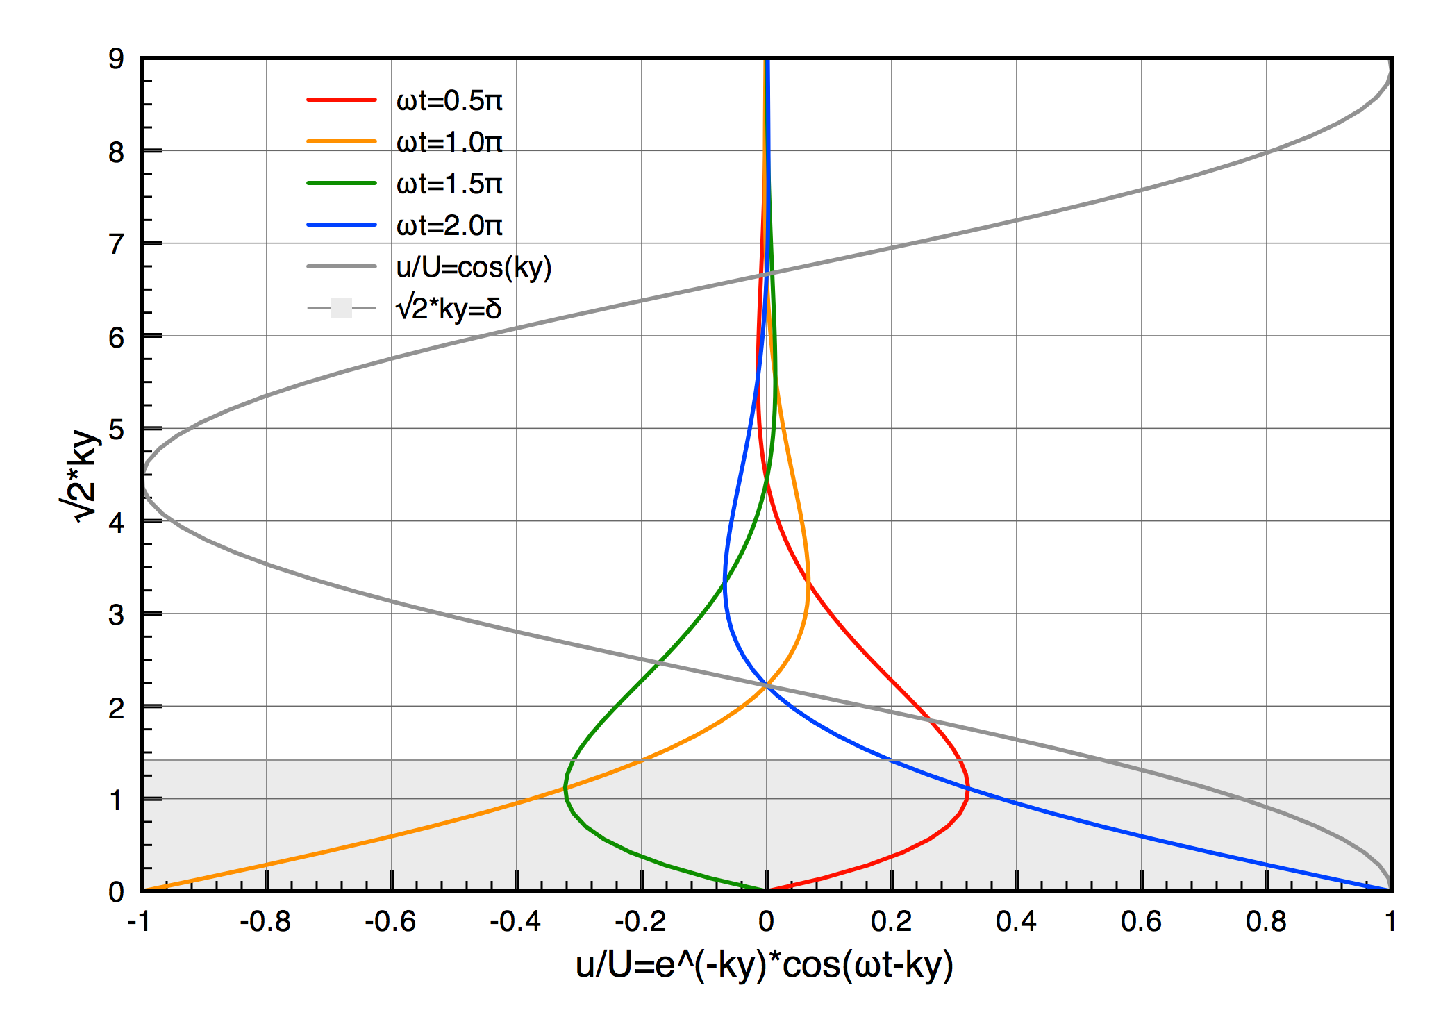
\includegraphics[width=14cm]{stokes_exact_cos1.eps}
\end{center}
\caption{Stokesの振動流の厳密解}
\label{fig:stokes_exact}
\end{figure}

%
\subsubsection{計算問題の準備}
作動流体として水($\nu=1.004 \times 10^{-6}[m^2/s]$),
振動数を$f=0.05[Hz]$,角振動数を$\omega=2\pi f=0.314[rad/s]$と考えると,
\textbf{式(\ref{eq:delta})}から,境界層厚さ,$\delta$は,2.5[mm]程度と算出される.
本計算では,$y$軸方向は,さらに減衰するまで,具体的には,10$\delta=2.5$[cm]以上の領域を,時間的には2周期,$\omega t=4\pi$まで計算することとした.

%
\subsubsection{計算領域と計算パラメータ}
「Rect」クラスの解析モデルは,全体領域を「Domain\_Info」タグで,2次元,3次元の別を「Intrinsic\_Example」タグで指定する.コンフィギュレーションファイル内の組込モデル名は,以下に示すように「Rectangular」である.\\
\hspace{1cm} $<$Param dtype="STRING" name="Example" value="Rectangular"/$>$\\

計算領域は,$-1.28\times 10^{-2}$[m]$\leq x \leq1.28\times 10^{-2}$[m],$0.00$[m]$\leq y \leq2.80\times 10^{-2}$[m],$-0.5\times 10^{-4}$[m]$\leq z \leq2.5\times 10^{-4}$[m],格子間隔は,$1.00\times 10^{-4}$[m],格子数を$256\times280\times3$として$z$方向に3層をとる,実質的2次元空間である.
総セル数は,215,040.$y=0$のY\_minus境界を振動面とみなし,$z$方向には,周期境界条件を設けている.

計算に用いた物性値を\textbf{表\ref{table:stokes_bussei}}に示す.物性値は,常温の水の値を使用した.

\begin{table}[htbp]
\begin{center}
\caption{計算に用いた物性}
\label{table:stokes_bussei}
\begin{tabular}{lccl}
\toprule
物性	&&物性値 &[単位]\\
\hline
動粘性係数& $\nu$&$1.004\times 10^{-6}$ & [m$^2$/s] \\
\bottomrule
\end{tabular}
\end{center}
\end{table}

計算に用いた外部境界条件を\textbf{表\ref{table:stokes bci}}に示す.

\begin{table}[hdpt]
%\small
\caption{計算に用いた境界条件}
\label{table:stokes bci}
\begin{center}
\begin{tabular}{lll}
\toprule
位置&タグ	&条件 	\\
\hline
 X\_minus, \, X\_plus&Periodic & Simple \\
 Y\_minus&Specified\_Velocity & Harmonic \\
 Y\_plus&Traction\_Free &\\
Z\_minus, \, Z\_plus& Periodic & Simple \\
\bottomrule
\end{tabular}
\end{center}
\end{table}

CBCに組み込まれているHarmonic運動は,次式で表される.
\begin{equation}
u=U \sin(2\pi f t + \phi)+b
\end{equation}
本計算では,以下のように設定した.
\begin{eqnarray}
U & = & 1.8\times 10^{-2} \mbox{[m/s]}\nonumber\\
f & = & 0.05\mbox{[Hz]}\nonumber\\
\phi & = & 0.5 \pi\mbox{[radian]}\nonumber\\
b & = & 0.0\mbox{[m/s]}
\end{eqnarray}  

\subsubsection{計算環境}
本計算に利用した計算機環境とソフトウェアを\textbf{表\ref{tbl: stokes env}}に示す.

\begin{table}[htdp]
\small
\caption{計算機環境および利用ソフトウェア}
\begin{center}
\begin{tabular}{ll}\toprule
Computer & eX. COMPUTER エアロストリーム RA7J-G23/S\\
CPU & Intel Core i7-950 (4 Cores/CPU)$\times$2\\
Clock & 3.07 GHz\\
Memory & 12GB \\
Cache & 8 MB\\
OS & Linux kernel 2.6.32-25-generic, ubuntu 10.04.1\\ \hline
MPI & OpenMPI 1.4.3\\
V-Sphere & ver. 1.8.4\\
CBC & ver. 1.4.6\\
FlowBase & ver. 2.4.3\\ \hline
Compiler & Intel Compiler Composer XE(12.0) 2011.3.174 C++/Fortran\\
Compile Option & -O3\\
\bottomrule
\end{tabular}
\end{center}
\label{tbl: stokes env}
\end{table}

\subsubsection{計算方法}
計算は,Navier-Stokes方程式を基礎方程式とし,時間積分は一次精度Euler陽解法,解法アルゴリズムにはFractional Step法を用いた.また,対流項の計算スキームには,三次精度MUSCLスキームを用いた.

時間積分幅の決定に,CFL\_Reference\_Velocityを使用し,クーラン数を0.2と指定した.また,計算時間は,$\omega t=4\pi$,$\omega=0.1\pi$より,$t=40$[sec]とした.

代表長さは$L=1.28\times 10^{-2}$[m],代表速度は$U=1.8\times 10^{-2}$[m/s]とした,代表時間は$t_0=7.1\dot{1}\times 10^{-1}$[sec],レイノルズ数はRe=230となる,

\paragraph{サンプリングの指定}
速度の値は,$x=0, \, z=0$上の$y=0 \sim y_{max}$の範囲を128分割してサンプリングする.サンプリング時間間隔は,$\omega t=0.5\pi$,$t=5$[sec]=7.03125[-]とした.

\subsubsection{計算結果と厳密解の比較}
\textbf{図\ref{fig:stokes_hikaku}}に,$\omega t=2.5\pi, \, 3.0\pi, \, 3.5\pi, \, 4.0\pi$におけるCBCによる計算結果と,$\omega t=0.5\pi, \, 1.0\pi, \, 1.5\pi, \, 2.0\pi$における厳密解を比較する.

なお,sampling.log結果ファイルの出力には,無次元を指定した.速度の無次元化された値はそのまま使用できるが,長さの無次元値には注意が必要である.CBCでは,一般的な無次元化,
\[
y_0=\frac{y}{L}
\]
を採用しているため,ファイルには$y_0$の値が出力される.
本例題では,文献\cite{hino:74:fd}および\textbf{図\ref{fig:stokes_exact}}との整合性のため,
\[
y_1=\sqrt{2}ky
\]
による無次元化を使用するため,$y_0\rightarrow y_1$の変換が必要である.
\[
y_1=\sqrt{2}ky=\sqrt{2}kLy_0=\sqrt{2}\sqrt{\frac{\omega}{2\nu}}Ly_0=\sqrt{\frac{2\pi f}{\nu}}Ly_0=7.16\times y_0
\]

\begin{figure}[htbp]
\begin{center}
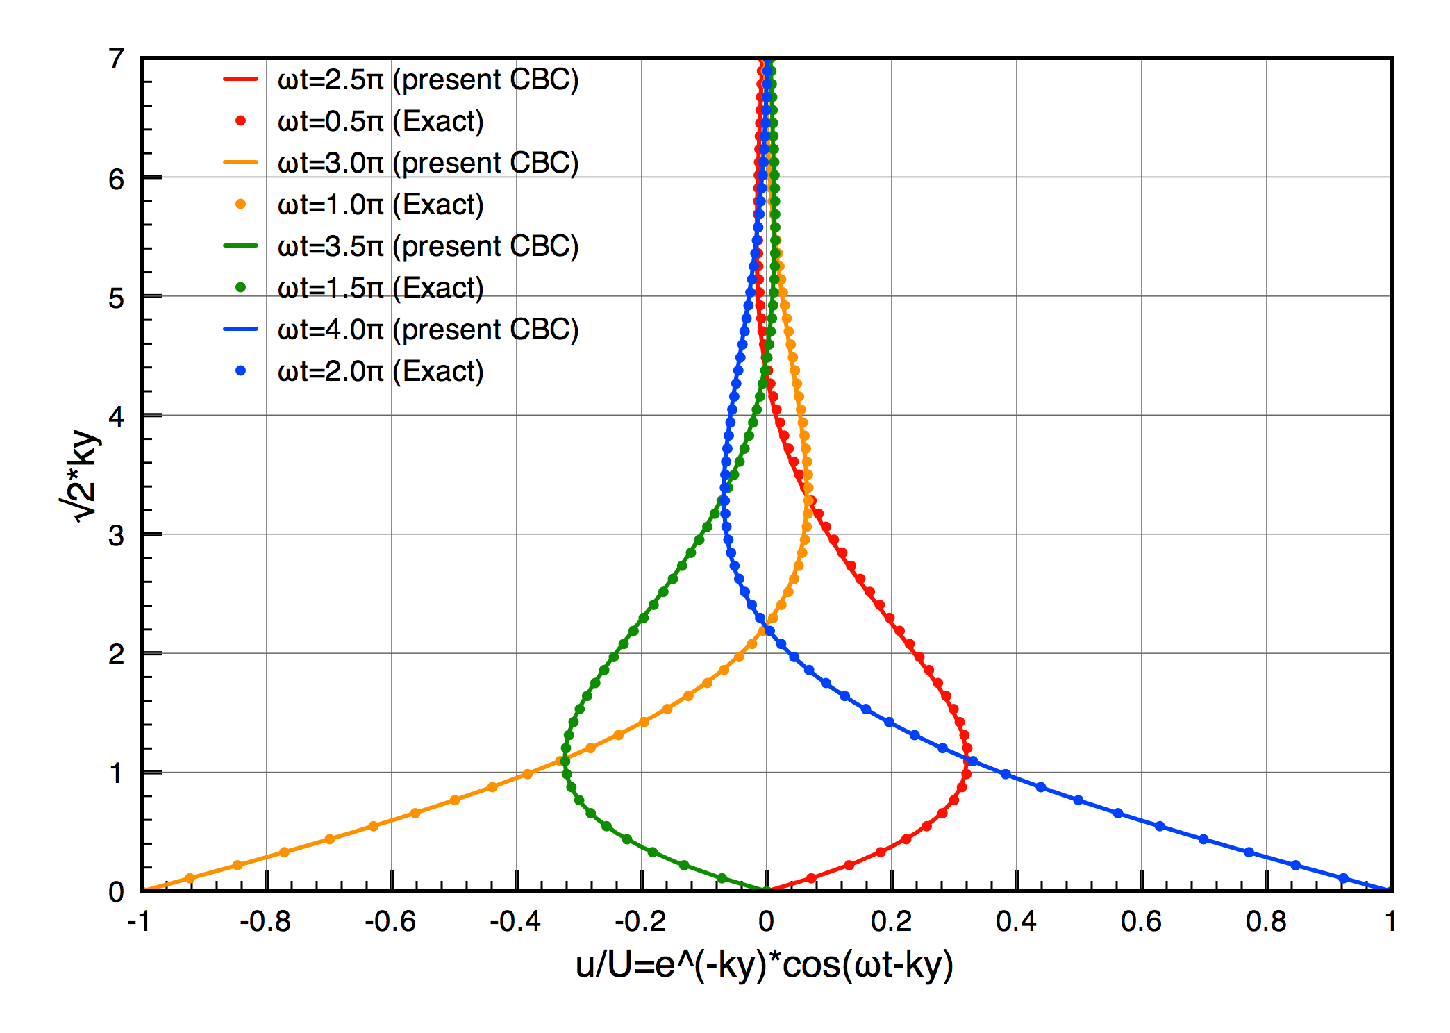
\includegraphics[width=14cm]{13stokes.eps}
\end{center}
\caption{Stokesの振動流の計算結果と厳密解の比較(計算2周期目)}
\label{fig:stokes_hikaku}
\end{figure}

CBCの計算結果は厳密解と非常によく一致しているように見える.しかしながら$\omega t=2,5\pi, \, 3.0\pi$では,
$\sqrt{2}ky\simeq 3$あたりで,僅かにずれている様子がわかる.

$\omega t=0.5\pi \sim 2.0\pi$ではCBCのずれはより大きい.
\textbf{図\ref{fig:stokes_hikaku1}}に,計算1周期目のCBCの結果と厳密解の比較を示す.

また,
CBCの計算結果の厳密解からの誤差を\textbf{図\ref{fig:stokes_error}}に示す.
時間を追うに従い,誤差が減少している様子がわかる.
1周期目(実線)では,$\omega t=0.5\pi$の最大誤差が厳密解の18.7\%,
2周期目(点線)では,$\omega t=2.5\pi$の最大誤差が厳密解の3.8\%,
$\omega t=4.0\pi$の最大誤差が厳密解の2.4\%である.
これらの誤差は,時間積分を一次精度Euler陽解法で行っていることが理由として考えられる.今後の課題として,時間積分の精度を上げて確認する予定である.

\begin{figure}[htbp]
\begin{center}
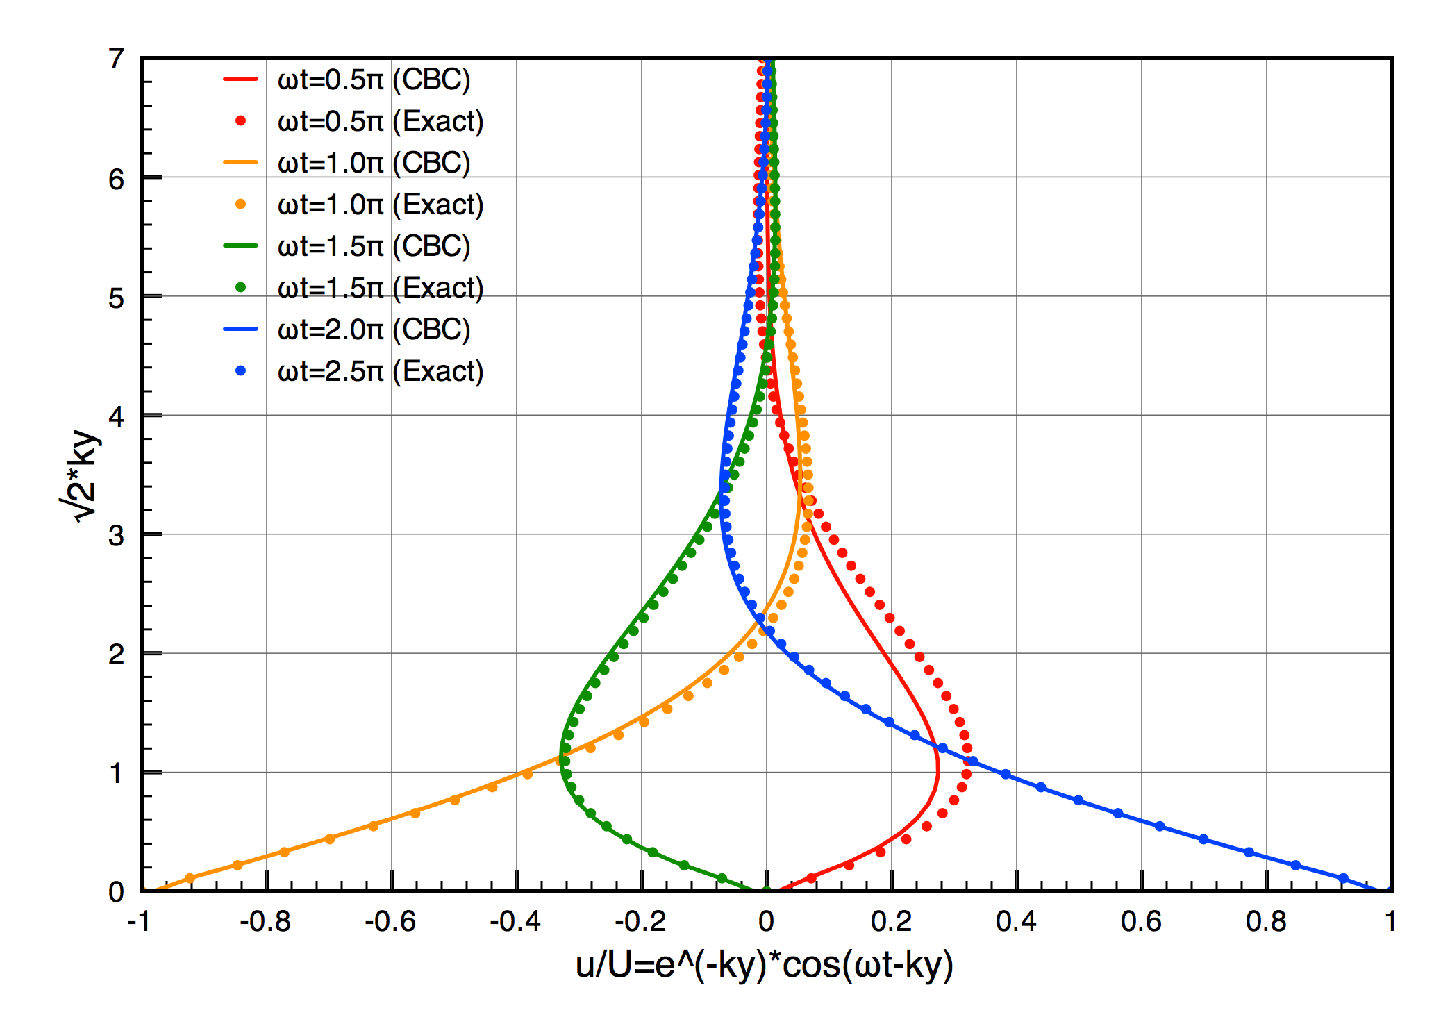
\includegraphics[width=14cm]{13-1stokes.eps}
\caption{Stokesの振動流の計算結果と厳密解の比較(計算1周期目)}
\label{fig:stokes_hikaku1}
%\end{figure}
%\begin{figure}[htbp]
%\centering
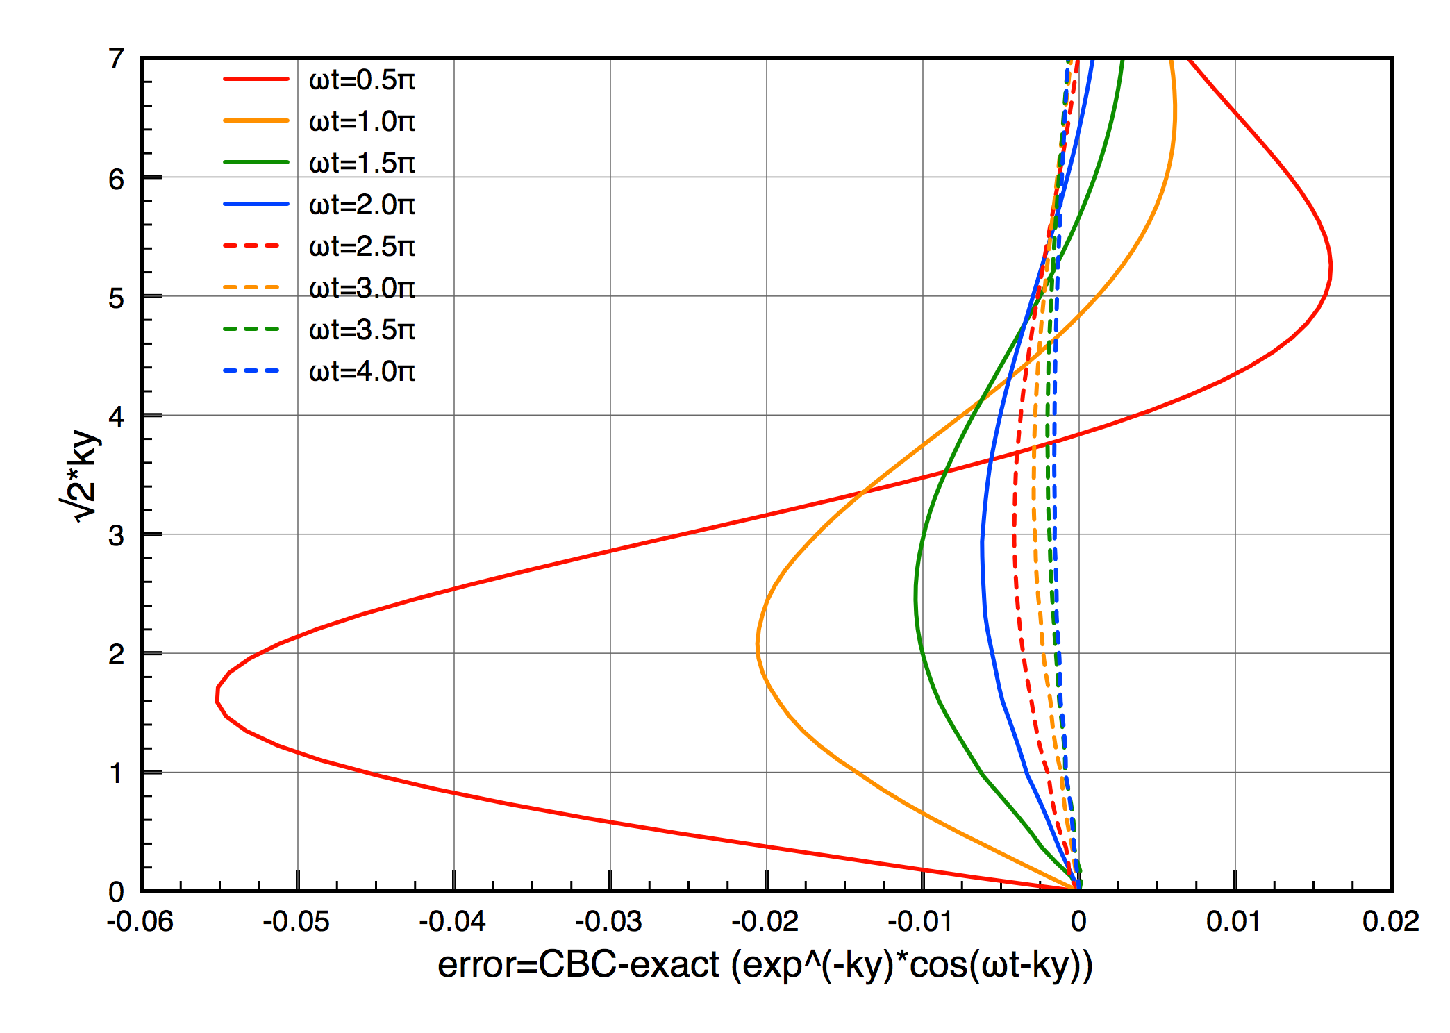
\includegraphics[width=14cm]{error1-2cycle.eps}
\caption{Stokesの振動流の計算結果の厳密解からの誤差}
\end{center}
\label{fig:stokes_error}
\end{figure}

\subsubsection{ファイルのメモ}
例題の提供ファイルの説明を以下に示す.
\begin{quote}
\begin{tabbing}
\hspace{15em}\= \hspace{20em}\kill
stokes.xml\> コンフィギュレーションXMLファイル\\
condition.txt \> 計算開始時conditionファイル\\
DomainInfo.txt \> 計算領域情報ファイル\\
history\_base.log.zip \> 履歴ファイル(解凍時3.5MB)\\
profiling.txt \> 実行性能測定結果ファイル\\
sample\_x=0\_y.log \> x=0上y軸に沿ったサンプリングファイル\\
plotフォルダ\> \textbf{図\ref{fig:stokes_exact}}〜\textbf{図\ref{fig:stokes_error}}のPlotファイルを含むフォルダ\\
\>(\url{http://plot/micw.eu/})\\
stokes2ndQ.mov.zip\> t=0[-]から56[-]までの$x=0$における$u$ベクトルのムービー(解凍時1MB).\\
\>元データは計算により出力されるvel***.sphファイル.\\
\>Visio(\url{http://vcad-hpsv.riken.jp/})で可視化できる.\\
gosa.f90\>sample\_x=0\_y.logを読み込み,厳密解からのエラーを算出するFortranプログラム
\end{tabbing}
\end{quote}




%%%
\chapter{検証事例}
\label{chpt:validation}

{\begin{abstract}
本章では,実験結果や理論解との比較により,格子解像度に対するソルバーの予測精度などのガイドラインを示します.
\end{abstract}
\pagebreak

%%
\section{二次元問題}


%%
\section{三次元問題}
\begin{enumerate}
\item 直方体内のキャビティ流れ
\end{enumerate}

%

\graphicspath{{./fig_LDC112/}}

%
\subsection{直方体内のキャビティ流れ: LDC112}

\subsubsection{目的}
本例題は,辺の長さが$1:1:2$となる3次元キャビティフローの初期時間発展の問題である.Rectangular組み込み例題クラスの3次元モデルを用いて解析し,Guermond\cite{guermond:02:JFM}が行った実験およびFEMシミュレーションと比較することにより,CBCソルバーの精度を検証する.

\subsubsection{問題の定義}
辺の長さの比が$X:Y:Z=1:1:2$である直方体の,$Y$マイナス面壁を$X$マイナス方向に一定速度$U$でスライドしたときに直方体内の静止している流体に生じる三次元非定常流れである.

\subsubsection{計算領域と観測}
計算領域は,\textbf{図\ref{fig:LDC112}}に示すような直方体である.

\begin{figure}[htbp]
\centering
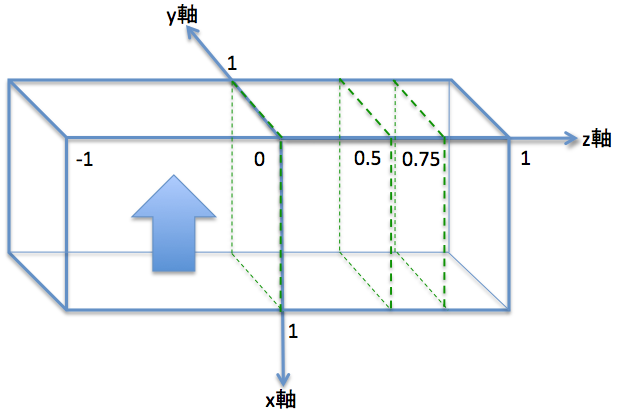
\includegraphics[width=12cm, bb=0 0 617 414]{LDC112.png}
\caption{計算領域の設定}
\label{fig:LDC112}
\end{figure}

$Y-$面は,$(u, v, w)=(-U, 0, 0)$のスライド壁,それ以外の$X\pm$面,$Y+$面,$Z\pm$面は,固定壁である.

流速ベクトルの観測は,$t = 4, \, 6, \,8, \,10, \,12$の無次元時刻に,$z = 0, \,0.5, \,0.75$の$xy$面内において行った.
%$Y$マイナス面以外はすべて固定壁.
%$Y$マイナス面(Lid)は$X$軸方向に無限に大きいとし,それが$X$軸マイナス方向に一定速度($U=1$)で滑ることにより誘起される(Driven),直方体(Cavity)内の流れの速度ベクトルを$z=0, \, 0.5, \, 0.75$において,$t=4, \, 6, \, 8, \, 10, \, 12$の時刻に観測した.

格子分割数は,$64\times 64 \times 128$である.

\subsubsection{計算環境}
本計算に利用した計算機環境とソフトウェアを\textbf{表\ref{tbl: LDC112 env}}に示す.

\begin{table}[htdp]
\small
\caption{計算機環境および利用ソフトウェア}
\begin{center}
\begin{tabular}{ll}\toprule
Computer & eX. COMPUTER\\
CPU & Intel Core i7-950 (4 Cores/CPU)\\
Clock & 3.07 GHz\\
Memory & 12GB \\
Cache & 8 MB\\
%Cache(3rd) & 4MB\\ 
OS & Linux ubuntu 2.6.32-25-generic\\ \hline
MPI & OpenMPI 1.4.3\\
V-Sphere & ver. 1.8.4\\
CBC & ver. 1.3.3\\
FlowBase & ver. 2.3.4\\ \hline
Compiler & Intel Compiler Composer XE(12.0) 2011.3.174 C++/Fortran\\
Compile Option & -O3\\
\bottomrule
\end{tabular}
\end{center}
\label{tbl: LDC112 env}
\end{table}

\subsubsection{解析モデルと計算パラメータ}
計算は,Guermondの実験を踏襲して,有次元のパラメータを入力して行った.
Navier-Stokes方程式を基礎方程式とし,時間積分は一次精度Euler陽解法,
解法アルゴリズムにはFractional Step法を用いた.
また,対流項の計算スキームには,三次精度MUSCLスキームを用いた.

解析モデルは,組み込み例題3次元のRectangularクラスから提供される(example.svx).

計算に用いたパラメータ(\textbf{表\ref{Table.paramLDC}}),流体の物性値(\textbf{表\ref{Table.busseiLDC}})などを示す.
\begin{table}[htbp]
\centering
\caption{計算に用いたパラメータ}
\label{Table.paramLDC}
\begin{tabular}{llll}\toprule
$h$ &短辺の長さ &$6.2\times10^{-2}$ &[m]\\
$U$ &$y=0$の壁面の移動速度 & $1.8\times10^{-2}$ &[m/s]\\
$\delta \tau $& 定速に達するまでの加速時間&$0.05$ &[s]\\
$\nu $ & クーラン数 & 0.1 & \\
\bottomrule
\end{tabular}
\end{table}

\begin{table}[htbp]
\centering
\caption{計算に用いた物性値}
\label{Table.busseiLDC}
\begin{tabular}{llll}\toprule
物性 &&物性値  & [単位]\\
\midrule
$\rho$ & 密度 & 998.2 & kg/m$^3$\\
$\mu$  & 粘性係数 & 1002.6 $\times 10^{-6}$ &[Pa $\cdot$ s]\\
\bottomrule
\end{tabular}
\end{table}

\subsubsection{サンプリングの指定}
\textbf{図\ref{fig:LDC112}}の$z=0, \, 0.5, \, 0.75$の$xy$面内において,$x=0.5, \, 0 \leq y \leq 1$の$x$方向の速度成分$u$, および$y=0.5, \, 0 \leq x \leq 1$の$y$方向の速度成分$v$を,$t=4, \, 6, \, 8, \, 10, \, 12$の無次元時刻にサンプリングした.

\subsubsection{解析結果}
計算結果のVelocity Profileを,Guermondによる実験値および有限要素法(FEM)でのシミュレーション結果と比較した.ここでは,$t=4$および$t=12$を\textbf{図\ref{fig:VP}}に示す.

Velocity Profileは,無次元で,$0.5-y$ に対する$ -0.5u$と,$0.5-x$ に対する$-0.5v$を同じ図にプロットすることにより作成している.

CBCの本解析結果は,Guermondの実験値,FEMの結果とよい一致を見せているといえる.

\begin{figure}[htdp]
\centering
\begin{minipage}{16cm}
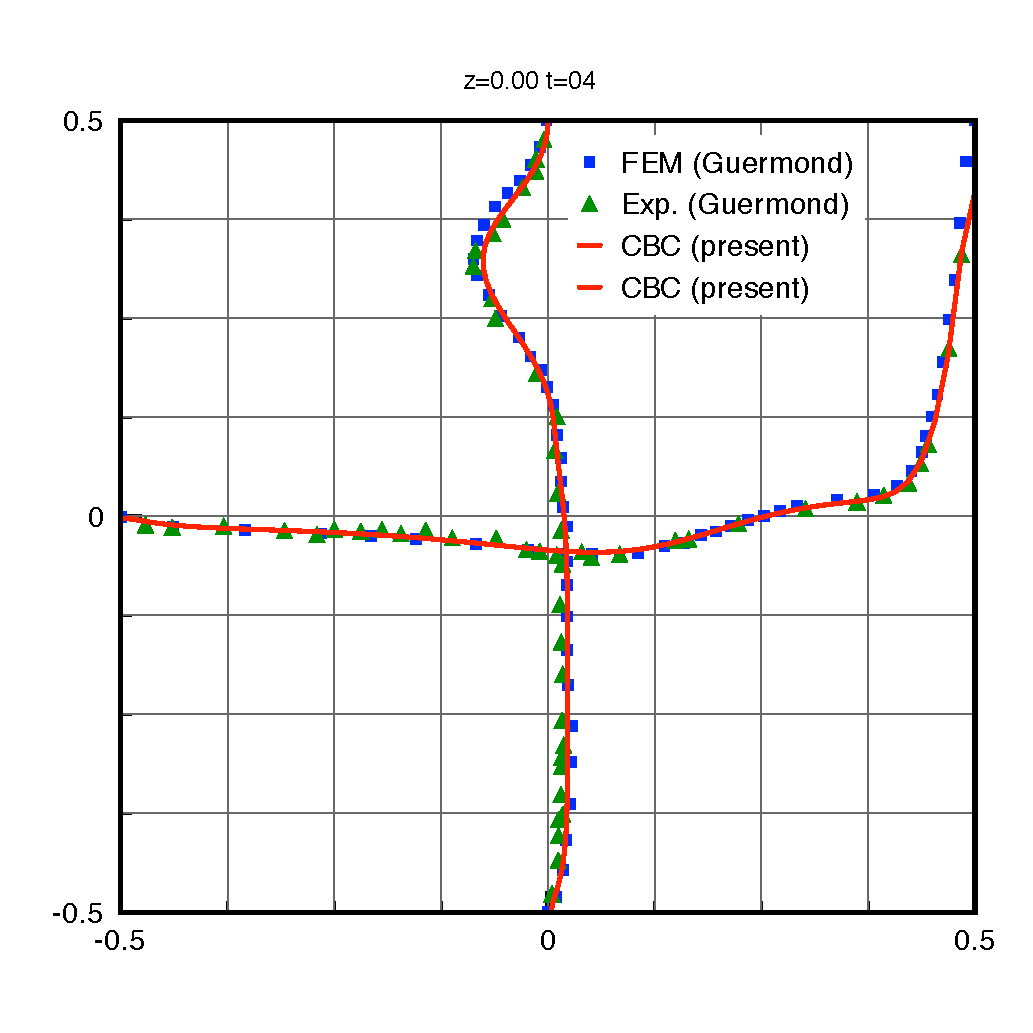
\includegraphics[width=8cm]{z00t04.eps}
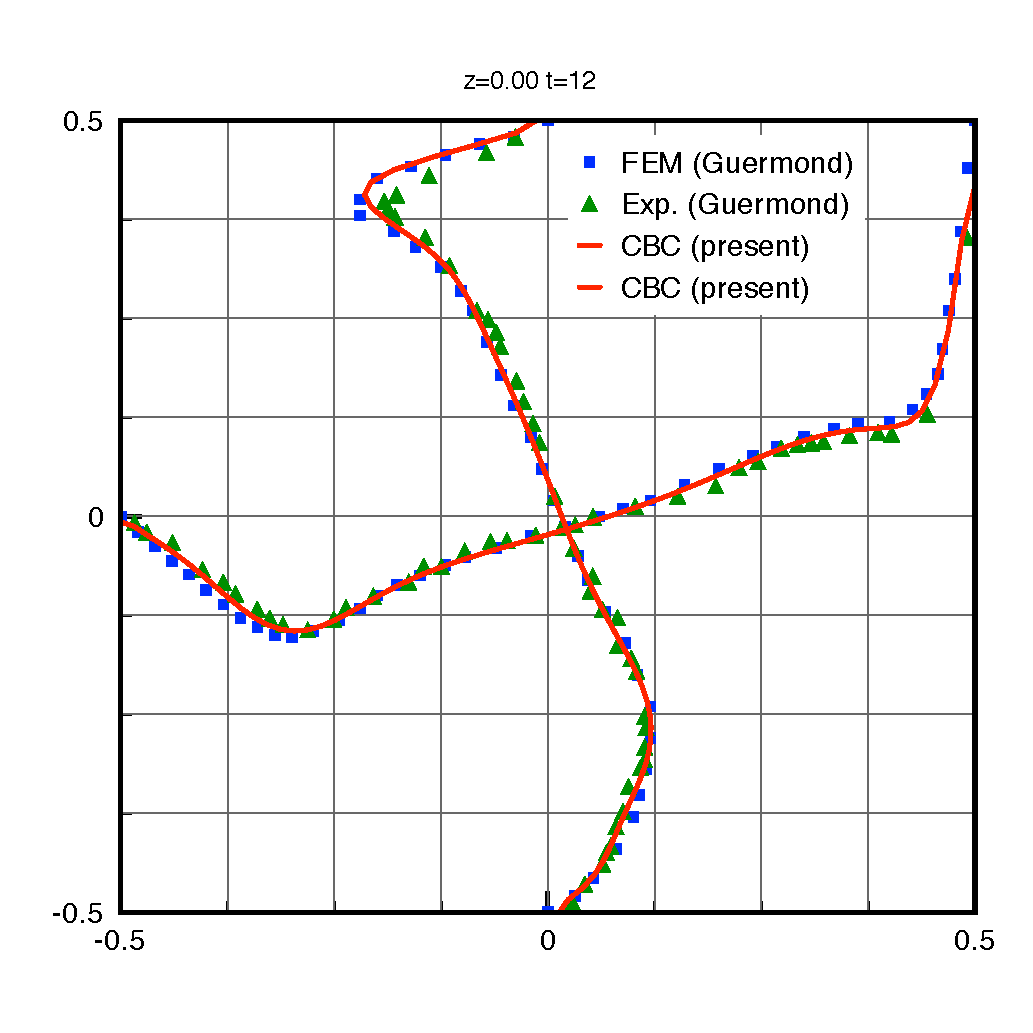
\includegraphics[width=8cm]{z00t12.eps}
\end{minipage}
\begin{minipage}{16cm}
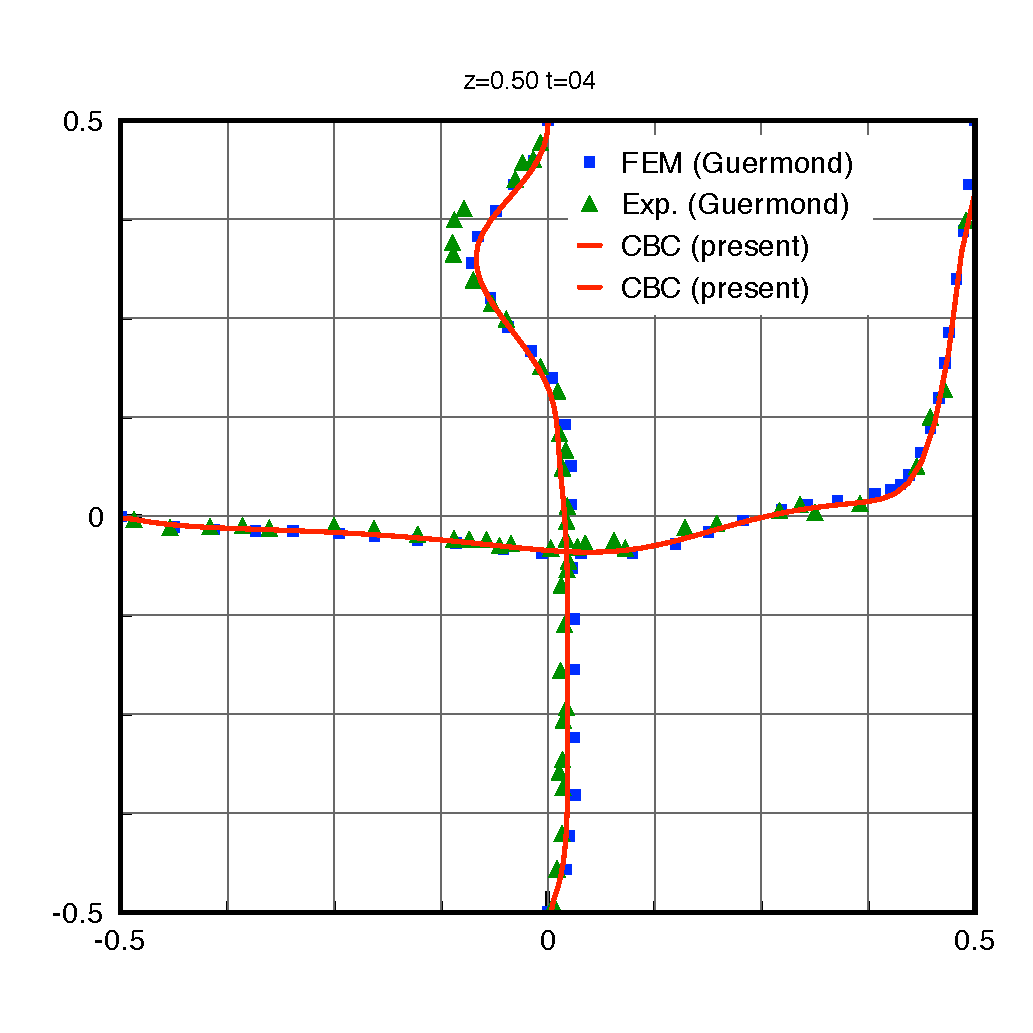
\includegraphics[width=8cm]{z50t04.eps}
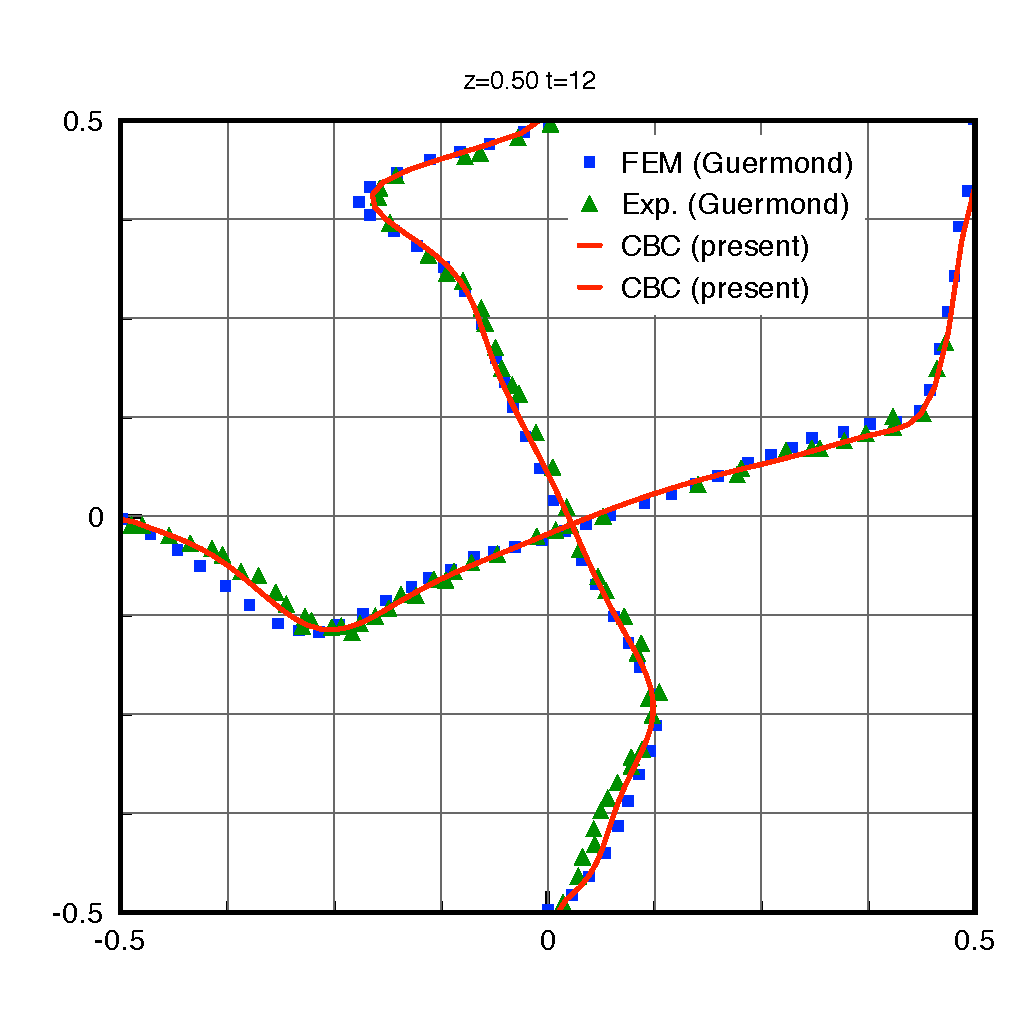
\includegraphics[width=8cm]{z50t12.eps}
\end{minipage}
\begin{minipage}{16cm}
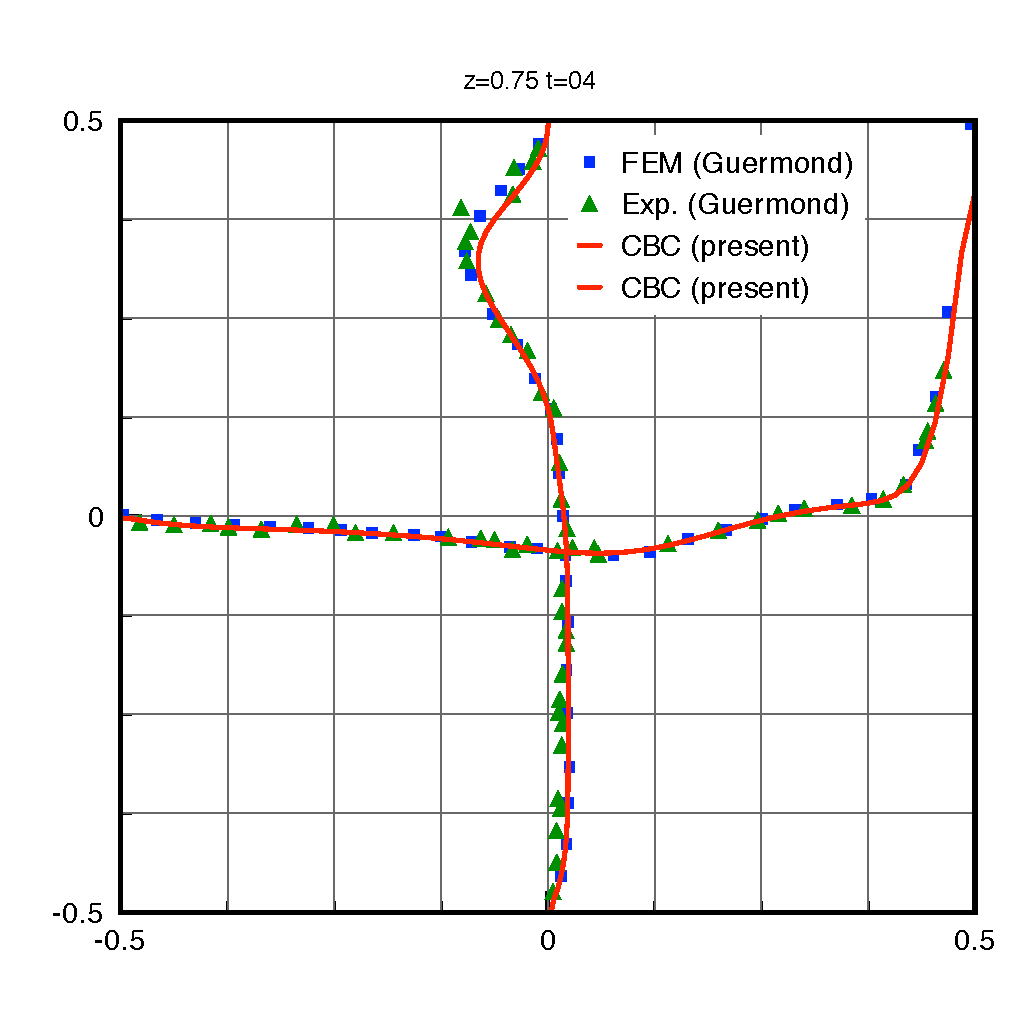
\includegraphics[width=8cm]{z75t04.eps}
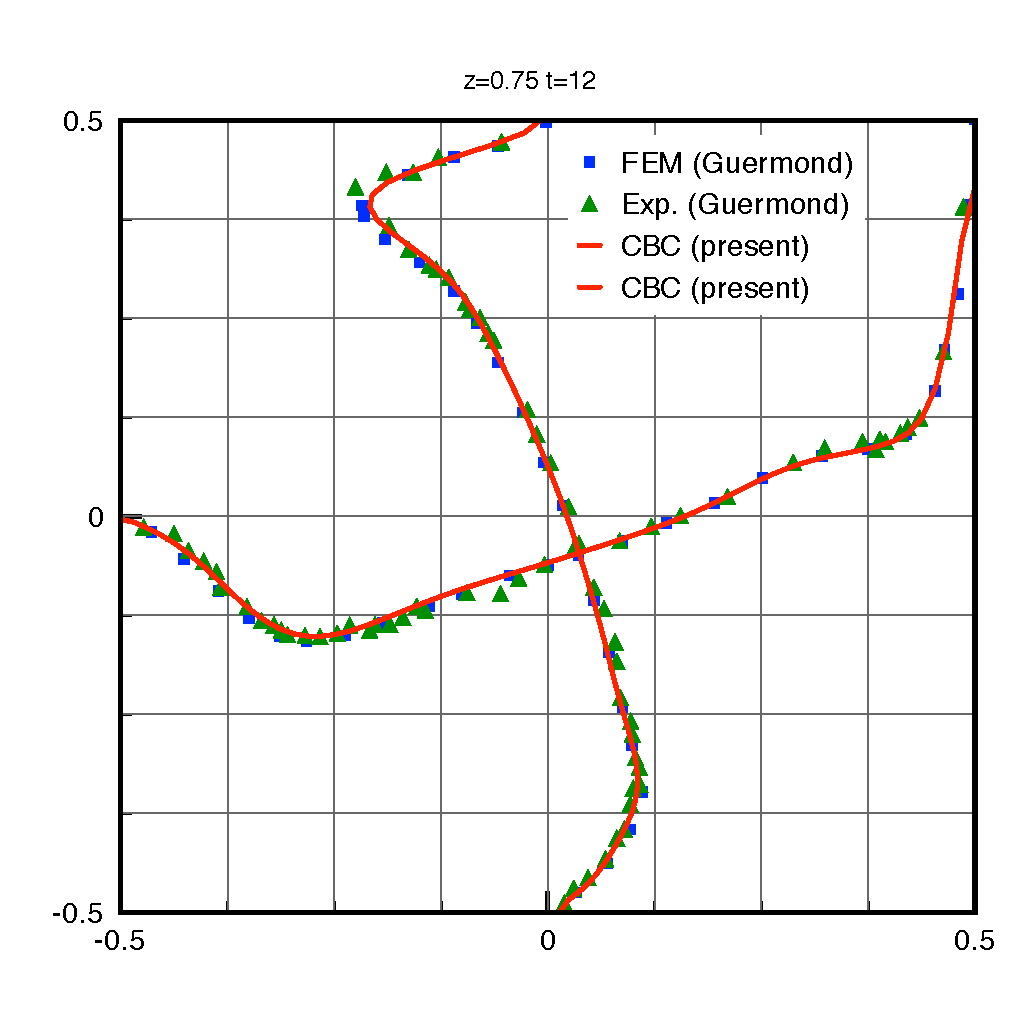
\includegraphics[width=8cm]{z75t12.eps}
\end{minipage}
\caption{$t=4$(左)と$t=12$(右)における$z=0, \, 0.5, \, 0.75$面のVelocity Profile}
\label{fig:VP}
\end{figure}

\subsubsection{ファイルのメモ}
例題の提供ファイルの説明を以下に示す.\\
\vspace{3mm}

\begin{tabularx}{180mm}{l@{}c@{}l@{}c@{}lX}
example\CID{07480}LDC112\, & \CID{07530}&\CID{00718}&\CID{07530}&sample\_\CID{00718}\_x.log & \CID{00718}($z=0,\,0.5,\,0.75$)の場合の$x$軸に沿ったsamplingファイル\\
&\CID{07482}&&\CID{07514}&sample\_\CID{00718}\_y.log & \CID{00718}($z=0,\,0.5,\,0.75$)の場合の$y$軸に沿ったsamplingファイル\\
&\CID{07482}&&\CID{07502}&\CID{00718}\CID{00734}.plot & \CID{00718}($z$情報), \CID{00734}($t$情報)のplotファイル(\url{http://plot.micw.eu/})\\
&\CID{07514}&\multicolumn{3}{l}{condition.txt} & conditionファイル\\
&\CID{07514}&\multicolumn{3}{l}{DomainInfo.txt} & 計算領域情報ファイル\\
&\CID{07514}&\multicolumn{3}{l}{example.svx.zip} & 出力された解析モデル圧縮ファイル\\
&\CID{07514}&\multicolumn{3}{l}{history\_base.log} & 履歴ファイル\\
&\CID{07514}&\multicolumn{3}{l}{ldc.xml} & コンフィギュレーションXMLファイル\\
&\CID{07502}&\multicolumn{3}{l}{profiling.txt} & 実行時性能測定結果ファイル
\end{tabularx}




%%%
\chapter{性能}
\label{chpt:performance}
{\begin{abstract}
本章では,計算性能に関するベンチマーク結果を示します.
\end{abstract}
\pagebreak

%

%
\graphicspath{{./fig_perf/}}

%%
\section{PMTクラス}

CBCソルバークラスには,組み込み例題として性能測定クラス(PMT class)を用意している.
PMT classは,三次元非圧縮流れのキャビティフロー問題を例題にした性能測定用の問題設定である.

具体的には,PMT classは次のような仕様としている.
\begin{enumerate}
\item 問題規模に関する入力は,VoxelSize, VoxelPitchの2つ.
\item 物理的にはキャビティフローを解く問題で,無次元パラメータを与える.
\item 圧力Poisson方程式の反復回数は指定回数で固定となる.
\item 不要なファイル入出力を抑制.
\item その他の提供機能オプションは利用可能.
\item FlowBaseクラス提供のPerfMonitorクラスでタイミングを測定し,統計結果をレポートする.
\end{enumerate}

性能に影響する主要なパラメータを以下に抜粋して示す.
{ \small
\begin{program}
<Steer>
  <Elem name="Algorithm">
    <Param dtype="STRING" name="Flow" value="FS_C_EE_D_EE"/>
  </Elem>
  <Elem name="Convection_Term">
    <Param dtype="STRING" name="Scheme" value="O3_MUSCL"/>
    <Param dtype="STRING" name="Limiter" value="Minmod"/>
  </Elem>
  <Elem name="Iteration">
    <Elem name="Flow">
      <Elem name="Poisson">
        <Param dtype="INT" name="Iteration" value="20"/>
        <Param dtype="REAL" name="Epsilon" value="1.0e-3"/>
        <Param dtype="REAL" name="Omega" value="1.2"/>
        <Param dtype="STRING" name="Norm" value="v_div_max"/>
        <Param dtype="STRING" name="Linear_Solver" value="SOR2SMA"/>
      </Elem>
    </Elem>
  </Elem>
  <Elem name="Log">
    <Param dtype="STRING" name="Unit_of_Log" value="Non_Dimensional"/>
    <Param dtype="STRING" name="Log_Base" value="On"/>
    <Param dtype="STRING" name="Log_Iteration" value="Off"/>
    <Param dtype="STRING" name="Log_Profiling" value="On"/>
    <Param dtype="STRING" name="Log_Wall_Info" value="Off"/>
    <Param dtype="STRING" name="Console_Interval_Type" value="Step"/>
    <Param dtype="REAL" name="Console_Interval" value="1"/>
    <Param dtype="STRING" name="History_Interval_Type" value="Step"/>
    <Param dtype="REAL" name="History_Interval" value="1"/>
  </Elem>
</Steer>
\end{program}
}

計算性能には,計算のカーネル部分だけでなく,境界条件処理部分の影響も大きい.
PMTクラスはキャビティフロー例題を利用しているので,必要なものは外部境界条件だけで,このコストは小さい.
実用的に利用される問題では,内部境界条件を導入することになる.
この内部境界条件は,空間的に局所的な処理となるので,並列計算時のロードバランスを崩す原因となる.
その影響は別途確認しておく必要がある.

%%
\subsection{測定パターン}
%
\subsubsection{Weak Scaling}
\textbf{表\ref{tbl:weak scaling plan}}に示すようなWeak scalingの性能測定を実施した.測定に予想される時間については,並列化率が99.4\%を仮定して,Amdhal則(\textbf{式(\ref{eq:amdhal's law})})から求めた\footnote{実際のコード並列化率は99.9\%以上だったので,測定時間は短かった.}.

\begin{equation}
\displaystyle { Speedup \, =\, \frac{1}{1-p+p/n} }
\label{eq:amdhal's law}
\end{equation}

\noindent ここでpは並列化率,nは並列数である.

\begin{table}[htdp]
\caption{Weak Scalingのテストケース}
\small
\begin{center}
\begin{tabular}{rrrrrrr}\toprule
\# of core & imax & jmax & kmax & Total \# of cell & Required memory [GB] & Expected run time [sec.]\\ \midrule
1    &  128 &  128 &  128 &   2.1M &    0.4 &   47.9\\
2    &  256 &  128 &  128 &   4.2M &    0.7 &   48.2\\
4    &  256 &  256 &  128 &   8.4M &    1.5 &   48.7\\
8    &  256 &  256 &  256 &  16.8M &    3.0 &   49.9\\
16   &  512 &  256 &  256 &  33.6M &    5.9 &   52.2\\
32   &  512 &  512 &  256 &  67.1M &   11.8 &   56.8\\
64   &  512 &  512 &  512 & 134.2M &   23.6 &   66.0\\
128  & 1024 &  512 &  512 & 268.4M &   47.2 &   84.3\\
256  & 1024 & 1024 &  512 & 536.9M &   94.5 &  121.1\\
512  & 1024 & 1024 & 1024 &  1074M &  188.9 &  194.6\\
1024 & 2048 & 1024 & 1024 &  2148M &  377.9 &  341.7\\
2048 & 2048 & 2048 & 1024 &  4295M &  755.7 &  635.8\\
4096 & 2048 & 2048 & 2048 &  8590M & 1511.4 & 1223.9\\
8192 & 4096 & 2048 & 2048 & 17180M & 3022.9 & 2400.3\\ \bottomrule
\end{tabular}
\end{center}
\label{tbl:weak scaling plan}
\end{table}

%
\subsubsection{Strong Scaling}



\pagebreak
%%
\section{計算機諸元}
%
\subsection{MacPro - Nehalem}

MacPro(Nehalem)の諸元を\textbf{表\ref{tbl:macpro-nehalem}}に示す\footnote{CPU情報はメニューバーのアップルマークの「このMacについて」および,コマンドライン\verb|$ /usr/sbin/system_profiler|,\url{http://ark.intel.com/Product.aspx?id=40200}から入手.}.

\begin{table}[htdp]
\caption{Specification of MacPro(Nehalem)}
\small
\begin{center}
\begin{tabular}{rl}\toprule
Processor & Intel Xeon E5520\\
\# of core & 4\\
\# of CPU & 2\\
Clock & 2.26 GHz\\
2nd cache & 256 kB (each core)\\
3rd cache & 8 MB (each proc.)\\
Peak FP rate Multi+Add & 4 flop/cycle\\
QPI speed & 5.86 GT/s (=23.44 GB/s)\\
Memory & DDR3-1066 (3ch.)\\ \bottomrule
\end{tabular}
\end{center}
\label{tbl:macpro-nehalem}
\end{table}

\textbf{図\ref{fig:nehalem}}にE5520プロセッサのアーキテクチャーを示す.

\begin{figure}[htdp]
\begin{center}
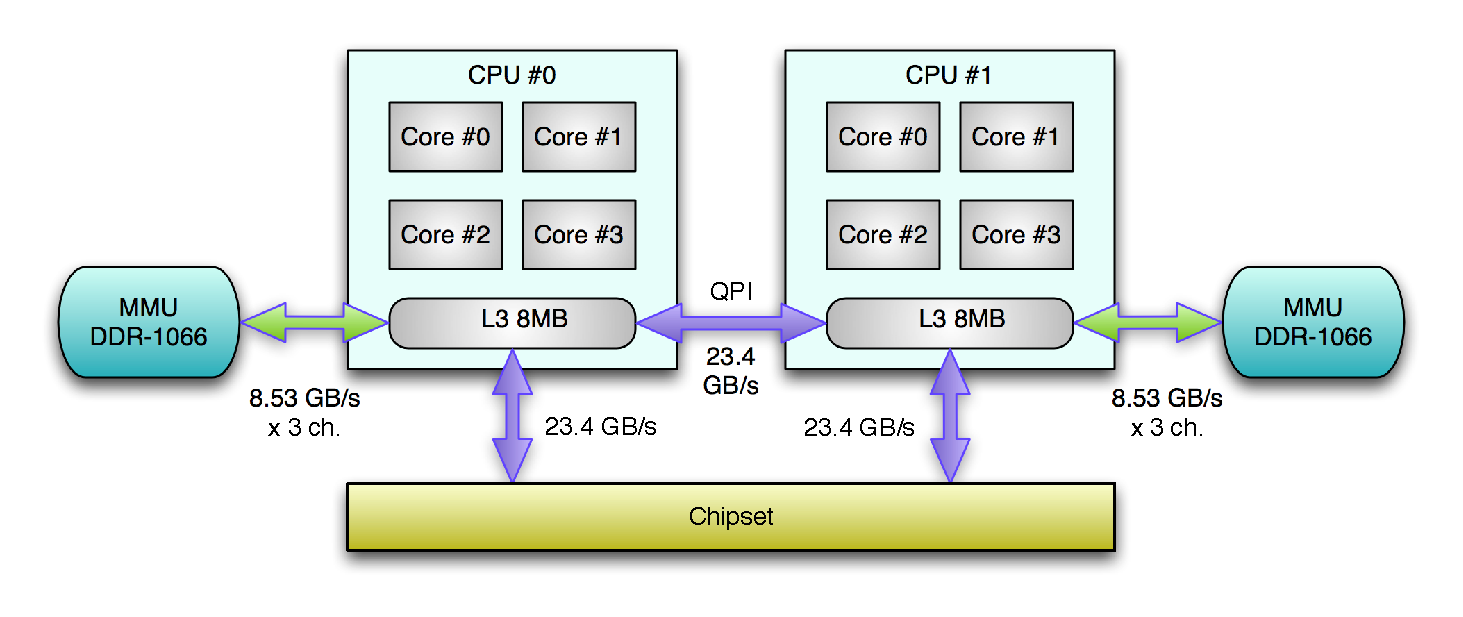
\includegraphics[width=14cm,clip]{E5520_arch.eps}
\end{center}
\caption{E5520のアーキテクチャー}
\label{fig:nehalem}
\end{figure}

QPIはQuickPath Interconnectで高速シリアルP2Pインターコネクトで,1リンク(片方向)あたり20bit(16bit-data, 2bit-protocol, 2bit-CRC error check)である\footnote{QPIはI/Oインターフェースではなく,システムはPCI-EをI/Oに利用する.}.
E5520のQPIは1リンクあたり5.86GT/sで,2リンク(双方向)時23.44GB/s$(=5.86\times 2B \times 2)$となる.
メモリバンド幅はDDR-1066(8.53GB/s)の3チャネルで,CPUあたり25.6GB/sとなる.

Nehalemコアの理論最大性能は1cycleあたり4浮動小数点演算が可能で,packed SSE(SIMD)命令により加算器と乗算器が同時に動作する場合にのみ達成される.
したがって,\hyperlink{tgt:perf prediction}{性能評価}で参照するCPUあたりのマシンバランス$B_M$は以下のようになる.

\begin{equation}
B_M \,=\, \frac{8.53\,GB/s \times 3\,ch.}{(4\,FLOP/cycle \times 2.26\,GHz) \times 4\,core} \,=\, \frac{25.6\,GB/s}{36.16\,GFLOPS} \sim 0.7\,B/F
\label{eq:B_M nehalem}
\end{equation}



%
\subsection{MacPro - Westmere}

MacPro(Westmere)の諸元を\textbf{表\ref{tbl:macpro-westmere}}に示す\footnote{\url{http://ark.intel.com/Product.aspx?id=47922}}.

\begin{table}[htdp]
\caption{Specification of MacPro(Westmere)}
\small
\begin{center}
\begin{tabular}{rl} \toprule
Processor & Intel Xeon X5650\\
\# of core & 6\\
\# of CPU & 2\\
Clock & 2.66 GHz\\
2nd cache & 256 kB (each core)\\
3rd cache & 12 MB (each proc.)\\
Peak FP rate Multi+Add & 4 flop/cycle\\
QPI speed & 6.4 GT/s (=25.6 GB/s)\\
Memory & DDR3-1333 (3ch.)\\ \bottomrule
\end{tabular}
\end{center}
\label{tbl:macpro-westmere}
\end{table}


\textbf{図\ref{fig:westmere}}にX5650プロセッサのアーキテクチャーを示す.

\begin{figure}[htdp]
\begin{center}
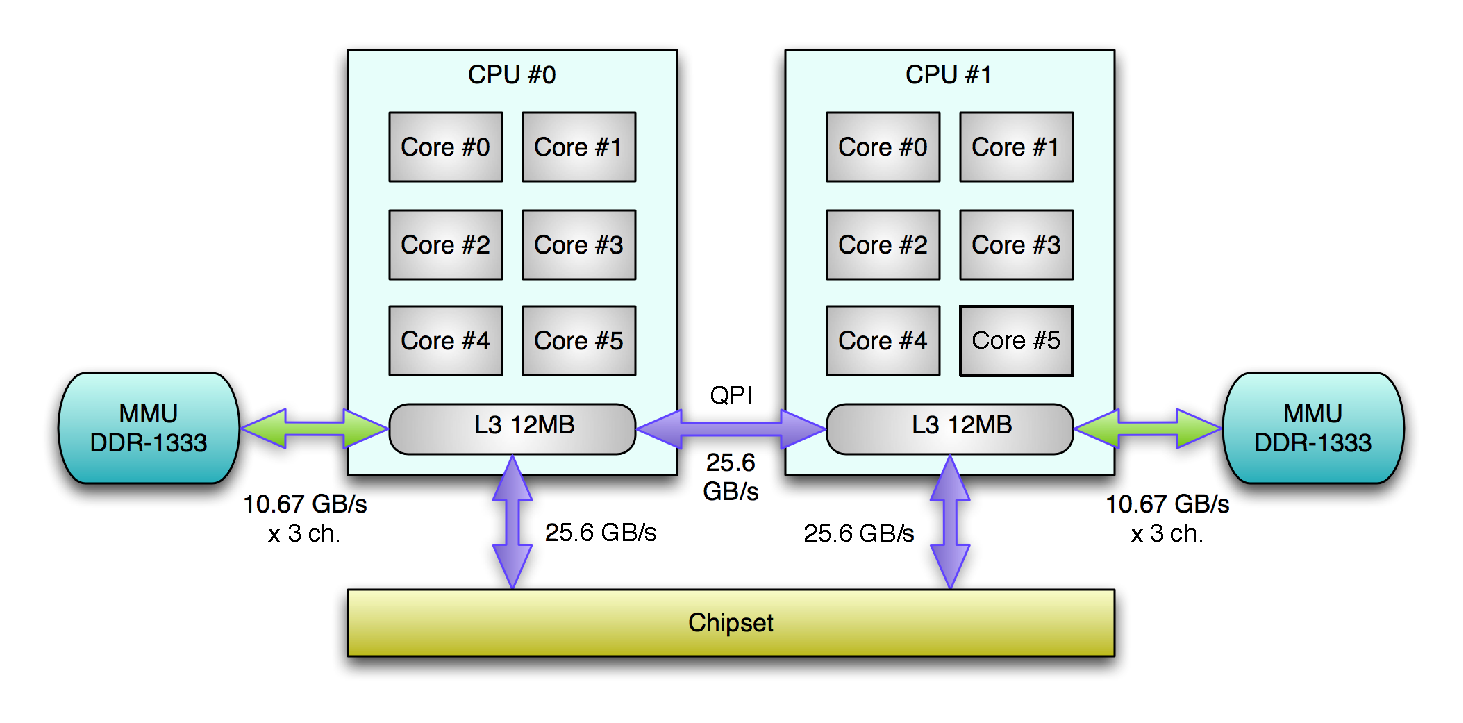
\includegraphics[width=14cm,clip]{X5650_arch.eps}
\end{center}
\caption{X5650のアーキテクチャー}
\label{fig:westmere}
\end{figure}

E5520と異なり,QPIは1リンクあたり6.4GT/sなので,双方向時にはQPI最大性能の25.6GB/sとなる.
また,メモリバンド幅はDDR-1333(10.67GB/s)なのでCPUあたり32GB/sである.
したがって,CPUあたりのマシンバランス$B_M$は以下のようになる.
NehalemよりもWestmereの方がByte/Flopは小さく,sustainedな計算には不利である.

\begin{equation}
B_M \,=\, \frac{10.67\,GB/s \times 3\,ch.}{(4\,FLOP/cycle \times 2.66\,GHz) \times 6\,core} \,=\, \frac{32.0\,GB/s}{63.84\,GFLOPS} \sim 0.5\,B/F
\label{eq:B_M westmere}
\end{equation}




%
\subsection{RICC}

RICC(Riken Integrated Cluster of Clusters)~\cite{ricc}の諸元を\textbf{表\ref{tbl:ricc}}に示す.
ネットワークにInfiniband x4 DDR\footnote{IB DDRは5Gbpsでデータ幅は8/10bitなので実質的に4Gbps=0.5GB/s.x4はその4倍で2GB/s.}を用いており,aggregate performanceは2TB/s,Bisection Bandwidthは240GB/sである.

\begin{table}[htdp]
\caption{Specification of RICC}
\small
\begin{center}
\begin{tabular}{rl}\toprule
Processor & Intel Xeon X5570\\
\# of core & 4\\
\# of CPU & 2\\
\# of Node & 1024\\
Clock & 2.93 GHz\\
2nd cache & 256 kB (each core)\\
3rd cache & 8 MB (each proc.)\\
Peak FP rate Multi+Add & 4 flop/cycle\\
QPI speed & 6.4 GT/s (=25.6 GB/s)\\
Memory & DDR3-1333 (3ch.)\\
Interconnect & IB x4 DDR (=2 GB/s)\\
Bisection bandwidth & 240 GB/s\\ \bottomrule
\end{tabular}
\end{center}
\label{tbl:ricc}
\end{table}


\begin{equation}
B_M \,=\, \frac{10.67\,GB/s \times 3\,ch.}{(4\,FLOP/cycle \times 2.93\,GHz) \times 4\,core} \,=\, \frac{32.0\,GB/s}{46.88\,GFLOPS} \sim 0.68\,B/F
\label{eq:B_M ricc}
\end{equation}

%
\subsection{FOCUS}
FOCUS~\cite{focus}の諸元を\textbf{表\ref{tbl:focus}}に示す.
バイセクションバンド幅は,x4 DDR双方向で$208nodes/2 \times 2GB/s \times 2\,=\,416\,GB/s$である.

\begin{table}[htdp]
\caption{Specification of FOCUS}
\small
\begin{center}
\begin{tabular}{rl}\toprule
Processor & Intel Xeon L5640\\
\# of core & 6\\
\# of CPU & 2\\
\# of Node & 208\\
Clock & 2.26 GHz\\
2nd cache & 256 kB (each core)\\
3rd cache & 12 MB (each proc.)\\
Peak FP rate Multi+Add & 4 flop/cycle\\
QPI speed & 5.86 GT/s (=23.44 GB/s)\\
Memory & DDR3-1333 (3ch.)\\
Interconnect & IB x4 DDR (=2 GB/s)\\
Bisection bandwidth & 416 GB/s\\ \bottomrule
\end{tabular}
\end{center}
\label{tbl:focus}
\end{table}

\begin{equation}
B_M \,=\, \frac{10.67\,GB/s \times 3\,ch.}{(4\,FLOP/cycle \times 2.26\,GHz) \times 6\,core} \,=\, \frac{32.0\,GB/s}{54.24\,GFLOPS} \sim 0.59\,B/F
\label{eq:B_M focus}
\end{equation}

%
%\subsection{K}

\pagebreak

%%
\section{FlatMPIの性能測定結果}
CBCソルバークラスの実効性能を各計算機上で測定した.
並列実行はFlatMPIである.

%
\subsection{MacPro - Nehalem}
\textbf{表\ref{tbl:macpro-env-nehalem}}に実行環境とシステム性能を示す.
\textbf{図\ref{fig:mac-nehalem-perf}}から8コア時の性能は14.4GFLOPSなので,理論性能の20\%の実行性能である.

\begin{table}[htdp]
\caption{Execution environment of MacPro(Nehalem)}
\small
\begin{center}
\begin{tabular}{rl}\toprule
System peak performance & 72.3 GFLOPS\\
Compiler & Intel C/C++, Fortran 12.0.2.142\\
Compiler option & -O3\\
MPI library & OpenMPI 1.4.1\\
V-Sphere & 1.8.3\\
CBC & 1.3.1\\
FB & 2.3.3\\
OS & 10.6.7 (Darwin 10.7.0)\\
Date of measurement & 2010-12-16\\ \bottomrule
\end{tabular}
\end{center}
\label{tbl:macpro-env-nehalem}
\end{table}

\begin{figure}[htdp]
\begin{center}
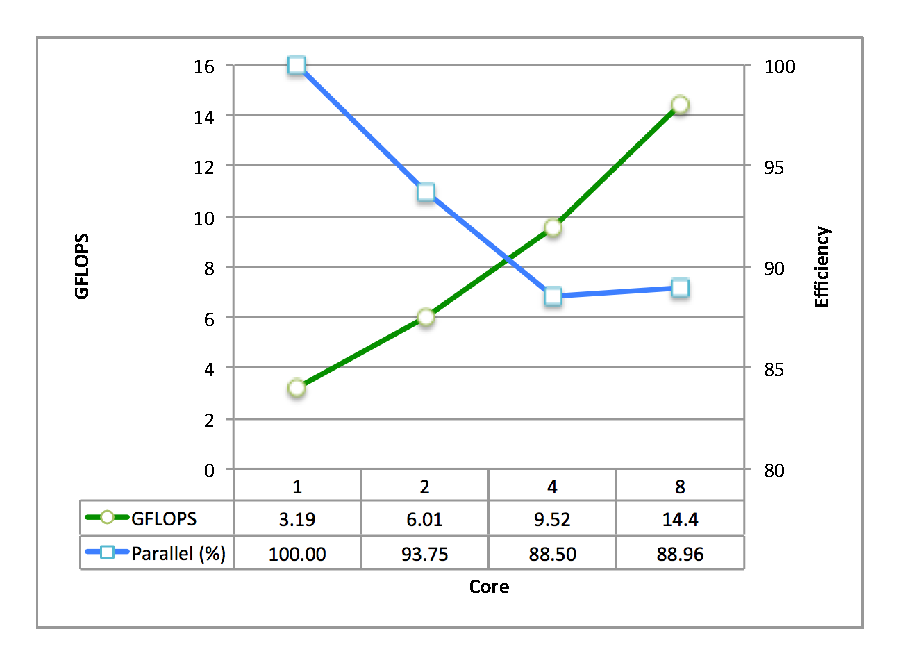
\includegraphics[height=8cm,clip]{mac-nehalem.eps}
\end{center}
\caption{MacPro(Nehalem)での実行性能}
\label{fig:mac-nehalem-perf}
\end{figure}

\pagebreak
%
\subsection{MacPro - Westmere}

\textbf{表\ref{tbl:macpro-env-westmere}}に実行環境とシステム性能を示す.
\textbf{図\ref{fig:mac-westmere-perf}}から12コア時の性能は18.6GFLOPSなので,理論性能の14.6\%の実行性能である.

Nehalemの場合も同様であるが,コア数が増える場合の並列性能の落ち込みは,MMU-CPU間のバンド幅におけるデータ供給量の飽和による.
CBCソルバークラスは,データ供給によって実効性能が制限される特性をもつ(Memory Bound).
マルチコア環境でアフィニティ制御を行わないと,プロセスはCPUのコアに詰めて割り振られる(デフォルトのポリシー).
この場合,CPU内で動いているコア数だけメモリへデータのダウンロード要求を出すのでメモリバンド幅は飽和し,相対的にデータ供給が低下し,性能劣化を引き起こす.
メモリへのデータの割り付けとコアのマッピングは制御していないので,場合によってはコアがリモートのメモリへアクセスすることもある.
その場合にはQPI経由になるので,データ転送速度はさらに低下する可能性がある.

\begin{table}[htdp]
\caption{Execution environment of MacPro(Westmere)}
\small
\begin{center}
\begin{tabular}{rl}\toprule
System peak performance & 127.7 GFLOPS\\
Compiler & Intel C/C++, Fortran 12.0.3.167\\
Compiler option & -O3\\
MPI library & OpenMPI 1.4.3\\
V-Sphere & 1.8.4\\
CBC & 1.3.5\\
FB & 2.3.6\\
OS & 10.6.8 (Darwin 10.8.0)\\
Date of measurement & 2011-06-28\\ \bottomrule
\end{tabular}
\end{center}
\label{tbl:macpro-env-westmere}
\end{table}

\begin{figure}[htdp]
\begin{center}
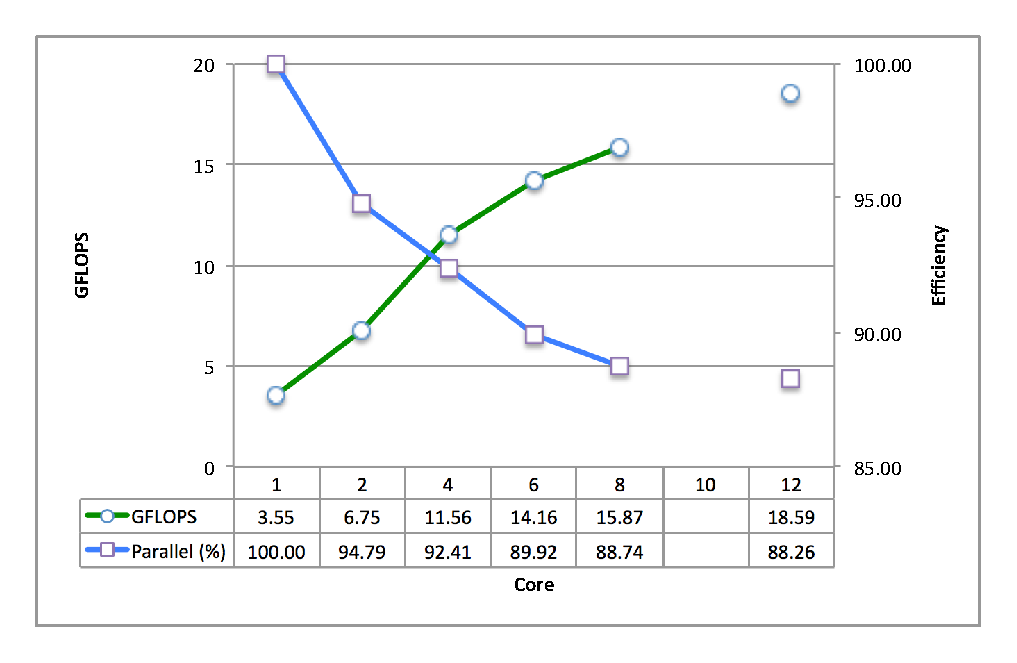
\includegraphics[height=8cm,clip]{mac-westmere.eps}
\end{center}
\caption{MacPro(Westmere)での実行性能}
\label{fig:mac-westmere-perf}
\end{figure}

\pagebreak
%
\subsection{RICC}

\textbf{表\ref{tbl:ricc-env}}にRICCの実行環境とシステム性能を示す.
\textbf{図\ref{fig:ricc-perf}}から8192コア時の性能は10TFLOPSなので,理論性能の10.4\%の実行性能である.


コア数が少ないところでの並列性能の落ち込みは,上述したようにノード内の帯域の問題である.
影響の現れ方は,コアへのプロセスマッピングポリシーに依存する.
各ノード内のコアが全て使われた状態でノード数が増加しているので,良好なスケーラビリティを見せている.

\begin{table}[htdp]
\caption{Execution environment of RICC}
\small
\begin{center}
\begin{tabular}{rl}\toprule
System peak performance & 96 TFLOPS\\
Compiler & Intel C/C++, Fortran 11.1.073\\
Compiler option & -O3\\
MPI library & OpenMPI 1.4.0?\\
V-Sphere & 1.8.3\\
CBC & 1.3.1\\
FB & 2.3.3\\
OS & RedHat\\
Date of measurement & 2011-02-28\\ \bottomrule
\end{tabular}
\end{center}
\label{tbl:ricc-env}
\end{table}

\begin{figure}[htdp]
\begin{center}
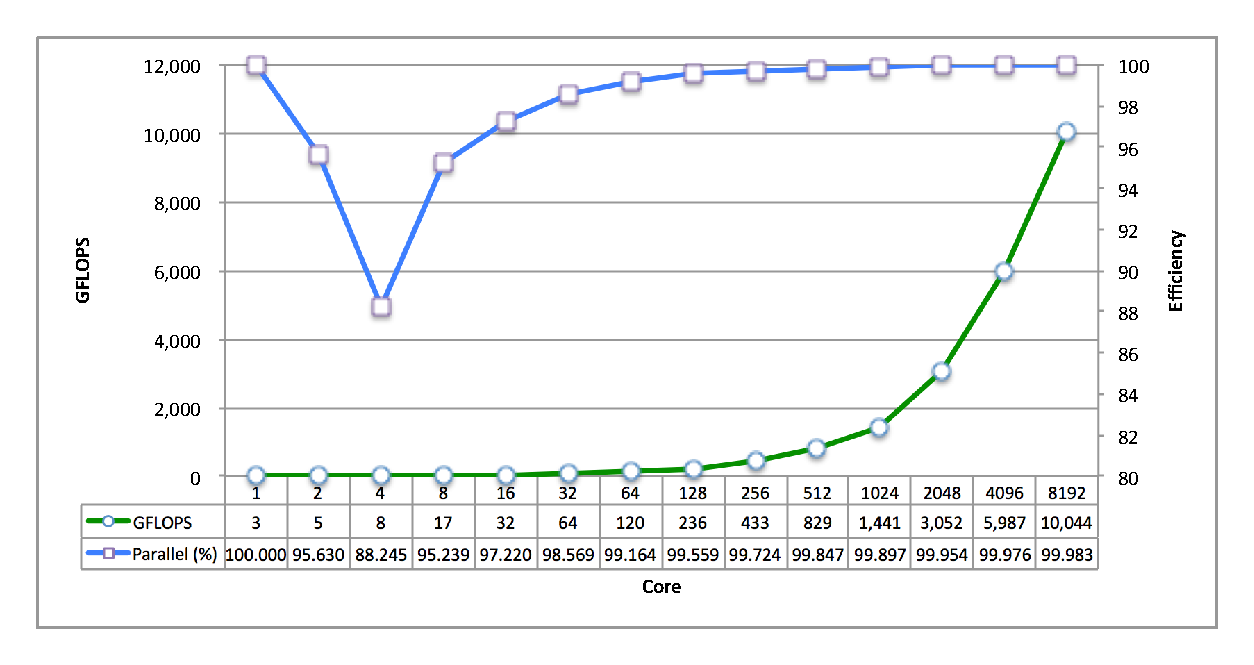
\includegraphics[height=8cm,clip]{ricc.eps}
\end{center}
\caption{RICCでの実行性能}
\label{fig:ricc-perf}
\end{figure}

\pagebreak
%
\subsection{FOCUS}

\textbf{表\ref{tbl:focus-env}}にRICCの実行環境とシステム性能を示す.
利用できるコア数は64ノード(768コア)なので,その場合のシステム性能は6943GFLOPSである.
\textbf{図\ref{fig:focus-perf}}から768コア時の性能は1036GFLOPSなので,理論性能の14.9\%の実行性能である.

\begin{table}[htdp]
\caption{Execution environment of FOCUS}
\small
\begin{center}
\begin{tabular}{rl}\toprule
System peak performance & 22.6 TFLOPS / 208nodes (6942.7 GFLOPS / 64 nodes)\\
Compiler & Intel C/C++, Fortran 12.0.084\\
Compiler option & -O3\\
MPI library & OpenMPI 1.4.1\\
V-Sphere & 1.8.4\\
CBC & 1.3.1\\
FB & 2.3.3\\
OS & Cent OS, Linux Kernel 2.6\\
Date of measurement & 2011-04-08\\ \bottomrule
\end{tabular}
\end{center}
\label{tbl:focus-env}
\end{table}

\begin{figure}[htdp]
\begin{center}
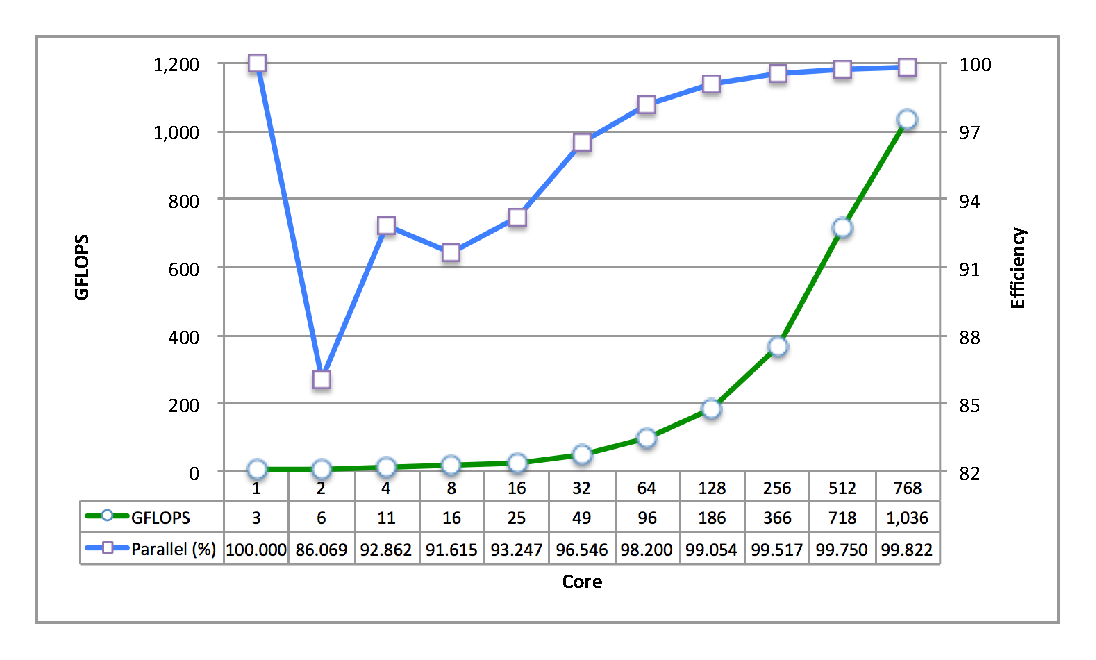
\includegraphics[height=8cm,clip]{focus.eps}
\end{center}
\caption{FOCUSでの実行性能}
\label{fig:focus-perf}
\end{figure}

\pagebreak
%%
\hypertarget{tgt:perf prediction}{\section{性能評価}}
%
\subsection{Machine Balance}



た\cite{treibig:10:springerlink}




%%%
\chapter{アップデート情報}
\begin{abstract}
本例題集のアップデート情報について記します.
\end{abstract}


{
\small

%
\subparagraph{Version 1.3.0\hspace{1cm}2011/09/14}

\begin{description}
\begin{indentation}{3zw}{0zw}
\item[-] クエット流とポアズイユ流を追記しました.
\end{indentation}
\end{description}
\vspace{2mm}

%
\subparagraph{Version 1.2.0\hspace{1cm}2011/06/28}

\begin{description}
\begin{indentation}{3zw}{0zw}
\item[-] 性能を追記しました.
\end{indentation}
\end{description}
\vspace{2mm}

%
\subparagraph{Version 1.1.0\hspace{1cm}2011/06/20}

\begin{description}
\begin{indentation}{3zw}{0zw}
\item[-] LDC112の例題を追加しました.
\item[-] 目次をサブセクションまで表示するように変更しました.
\end{indentation}
\end{description}
\vspace{2mm}

%
\subparagraph{Version 1.0.0\hspace{1cm}2011/01/12}

\begin{description}
\begin{indentation}{3zw}{0zw}
\item[-] 例題集のひな形を作成しました.
\end{indentation}
\end{description}

}




%%%
\bibliographystyle{junsrt}
\bibliography{vv}

\newpage
\printindex
%
%
\end{document}